\documentclass[report.tex]{subfiles}

\begin{document}

\chapter{Software Part}

\section{Small Watch Application Development}

The second biggest task of of this project is to develop a simple watch application for the prototype board of \textit{LTEWatch}. Due to the limited time available for the project, the objectif is not to develop a definitive and complex smart-watch application but is to implement every functional blocks from the prototype board, because of this, the developed application is name "\textit{PicoWatch}".\\

Following the system functional decomposition (p.:\pageref{sec:sys_func_dec}), the small watch application 
(\textit{PicoWatch}), is decomposed in the following functional blocks:

\begin{enumerate}
\item \textbf{Power Supply}: Relating to battery and charger module
\item \textbf{User Interface}: Relating to user-accessible peripherals and sensors
\item \textbf{RF \& Network}: Relating to \textit{LTE-M/NB-IoT}, \textit{MQTT} and \textit{GNSS}
\item \textbf{Debugging}: Relating to \textsc{VS-Code} \textit{IDE} logging
\end{enumerate}

\section{\textit{LTEWatch} Application Decomposition} \label{sec:ltewatch_app_decomp}

\subsection{Power Supply Block:}
\subsubsection{Description:}
This block integrates the battery charger module and the battery level monitoring unit of the \textit{LTEWatch} prototype board and should implement the features listed below:

\begin{enumerate}
\item \textbf{Battery Charger:}
\begin{itemize}
\item Set battery charger's configurable registers;
\textit{Battery Voltage Control}, \textit{- Fast Charge Current Control}, \textit{- Charger Control}, \textit{- Input Current Limit Control}, \textit{- TS Control} and others
\item Get charger's interruption flags
\item Read and clear charger's status and fault registers; \textit{Charger Status}, \textit{- Charger Status and Faults} and \textit{- Charger Flag Registers }
\end{itemize}
\item \textbf{Batter Level Monitoring:}
\begin{itemize}
\item Measure and store battery voltage level value in "\si{\milli\volt}"
\item Convert and store battery level value to "\si{\percent}"
\end{itemize}
\end{enumerate}

\pagebreak

\subsection{User Interface Block:}
\subsubsection{Description:}
This block integrates all the peripherals and sensors accessible to the user of the \textit{LTEWatch} prototype board. The \textit{User Interface Block} is the only way users interact with the device, which includes:
\begin{itemize}
\item \textbf{Output interactions:} "\textit{DEVICE}" $\rightarrow$ "\textit{USER}", such as:
\begin{itemize}
\item display time using clock hands,
\item display device information using the LCD and LEDs.
\end{itemize}   
\item \textbf{Input interactions:} "\textit{USER}" $\rightarrow$ "\textit{DEVICE}", such as:
\begin{itemize}
\item Change modes or settings of the device using buttons and accelerometer.
\end{itemize}   
\end{itemize}
This block should implement the features listed below:
 
\begin{enumerate}
\item \textbf{Buttons:}
\begin{itemize}
\item Get button press and button release action events
\item Filter button events with debounce
\item Convert button events into button action; \textit{Click}, \textit{- Double Click}, \textit{- Triple Click}, \textit{- Long-Press} and \textit{- Double Long-Press}
\end{itemize}
\item \textbf{LEDs:}
\begin{itemize}
\item Set \textbf{\textcolor{mygreen}{ON}}/\textbf{\textcolor{red}{OFF}},
\item \textbf{\textcolor{mygreen}{START}}/\textbf{\textcolor{red}{STOP}} Blinking
\end{itemize}
\item \textbf{Display:}
\begin{itemize}
\item Interface with \textsc{SHARP} \textit{Memory-In-Pixel (MIP)} LCD
\item Display modes; \textit{Set Motor Position Mode}, \textit{- Set GNSS Antenna Mode}, \textit{- LTEWatch Mode} and \textit{GNSS Tracking Mode}
\item Display device information; \textit{Date}, \textit{- Current Time}, \textit{- LTE/MQTT Connection State}, \textit{- GNSS Connection State}, \textit{- Current Battery Level} and \textit{- Battery Charging State}
\end{itemize}
\item \textbf{Motorized Clock Hands:}
\begin{itemize}
\item Move stepper motors position
\item Set stepper motors position
\item Get current stepper motors position
\item Display time on stepper motors; \textit{Hour}, \textit{- Minute}, \textit{- Second}
\end{itemize}
\item \textbf{Accelerometer\footnote{Optional: Depending on available time}:}
\begin{itemize}
\item Read 3-axis accelerometer values
\item Convert accelerometer acceleration values to speed
\item Add functionality; \textit{Wake-Up Event}, \textit{- Pedometer}, \textit{- Tracking Refresh-Rate Modification} and others.
\end{itemize}
\end{enumerate}

\subsection{RF \& Network Block:}
\subsubsection{Description:}
This block is one of the most important in the device, as it basically defines the name of the project. By integrating the \textit{LTE-M/NB-Iot} modem, the \textit{MQTT} client and the \textit{GNSS} receiver module of the \textit{LTEWatch} prototype board, this block should implement the following features:

\begin{enumerate}
\item \textbf{\textit{LTE-M/NB-Iot Modem}:}
\begin{itemize}
\item \textbf{\textcolor{mygreen}{Connect}}/\textbf{\textcolor{red}{Disconnect}} to/from \textit{LTE-M/NB-Iot} network
\item Set use of on-board or external \textit{LTE} antenna
\end{itemize}
\item \textbf{\textit{MQTT} Client:}
\begin{itemize}
\item \textbf{\textcolor{mygreen}{Connect}}/\textbf{\textcolor{red}{Disconnect}} client to \textit{MQTT} broker
\item Publish data on \textit{MQTT} broker topics
\item Subscribe to \textit{MQTT} broker topics\footnote{Optional: Depending on available time}
\end{itemize}
\item \textbf{\textit{GNSS} Receiver:}
\begin{itemize}
\item Set \textit{GNSS} receiver module configuration
\item Ask \textit{GNSS} receiver for position
\item Get and store \textit{GNSS} receiver communications (answers)
\item Set use of on-board or external \textit{GNSS} antenna
\end{itemize}
\end{enumerate}

\subsection{Debugging Block:}
\subsubsection{Description:}
The \textit{nRF COnnect SDK} development environment for \textsc{VS-Code} allows to transmit logs for debugging purposes. This can be achieved either using \textit{RTT} logging option using the \textit{J-Link} from \textsc{Segger} or eiter using \textit{UART} logging. The difference between the tow options is that \textit{UART} logging require target's log to pass through a \textit{FTDI} \textit{UART-to-USB} interface. In order to use \textit{UART} logging option, this block should implement the following modules.
\begin{enumerate}
\item \textbf{\textit{UART} Logging:}
\begin{itemize}
\item Interface with \textit{USB-to-UART} \textit{FTDI} interface module
\item Send data to \textit{FTDI} interface module
\item Get data from \textit{FTDI} interface module
\end{itemize}
\end{enumerate}

\pagebreak

\subsection{Application Functional Decomposition Diagram}

In order to have a more visual understanding of the application, it is interesting to decompose the application software in a functional block diagram that illustrates each block with its correspond pin assignment. With this diagram, it is easier to understand which \textit{API}, library and peripherals need to be implemented to integrate each features. \\

Figure \ref{fig:software_diag} illustrates the functional decomposition diagram of \textit{LTEWatch} application software:

\begin{figure}[H]
	\centering
	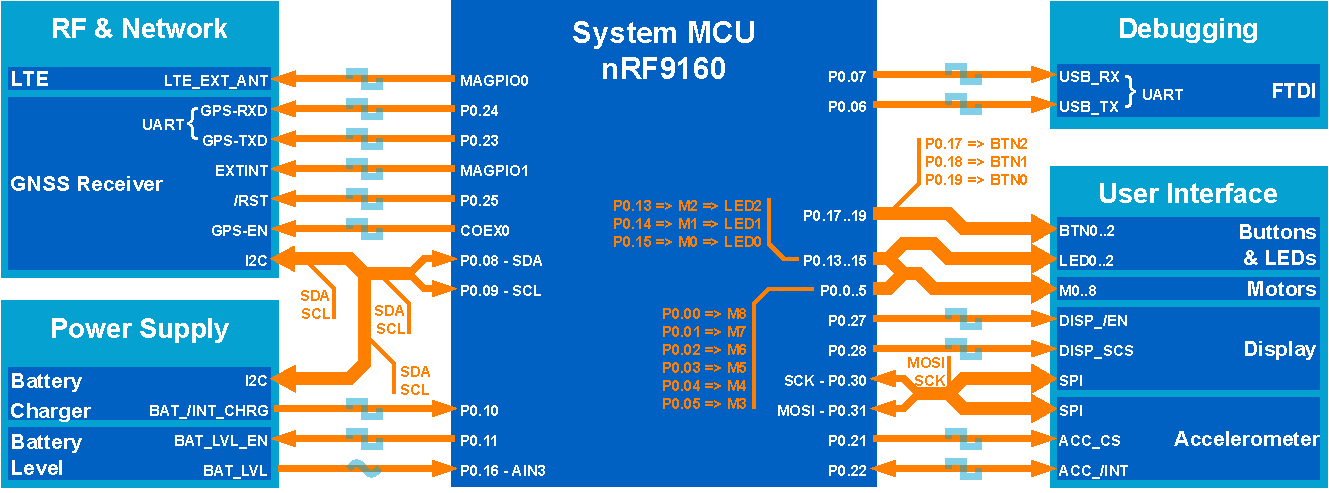
\includegraphics[width=1\textwidth]{Include/Figure/software/software_diag.pdf}
	\caption{\textit{LTEWatch} Application Functional Decomposition Diagram}
	\label{fig:software_diag}
\end{figure}

As shown in figure \ref{fig:software_diag}, even if the goal of the firmware development is to implement a small watch application to validate prototype board hardware and features, the \textit{LTEWatch} application (firmware) is already quite complex and requires to implement several  peripherals.\\

The small watch application firmware (\textit{LTEWatch}) require following peripherals to be implemented:
\begin{itemize}
\item many digital inputs and outputs for LEDs, motors and command signals,
\item several interrupt sensitive digital inputs for external modules and buttons,
\item an analog input (\textit{ADC}) for battery level monitoring (AIN3),
\item two \textit{UART} serial bus for the \textit{FTDI} interface and the \textit{GNSS} receiver,
\item a \textit{I2C} serial bus for the battery charger and the \textit{GNSS} receiver,
\item a \textit{SPI} serial bus for the display and the accelerometer,
\item and a \textit{LTE Modem} for \textit{LTE-M/NB-IoT} RF communication.
\end{itemize}

\pagebreak

\section{\textit{LTEWatch} Software Architecture}

As seen in the "\textit{LTEWatch Application Decomposition}" section starting at page \pageref{sec:ltewatch_app_decomp}, the developed application is relatively complex and integrates multiple components and features. For better understanding, a visual illustration of the developed firmware architecture is shown in figure \ref{fig:software_layers}:

\begin{figure}[H]
	\centering
	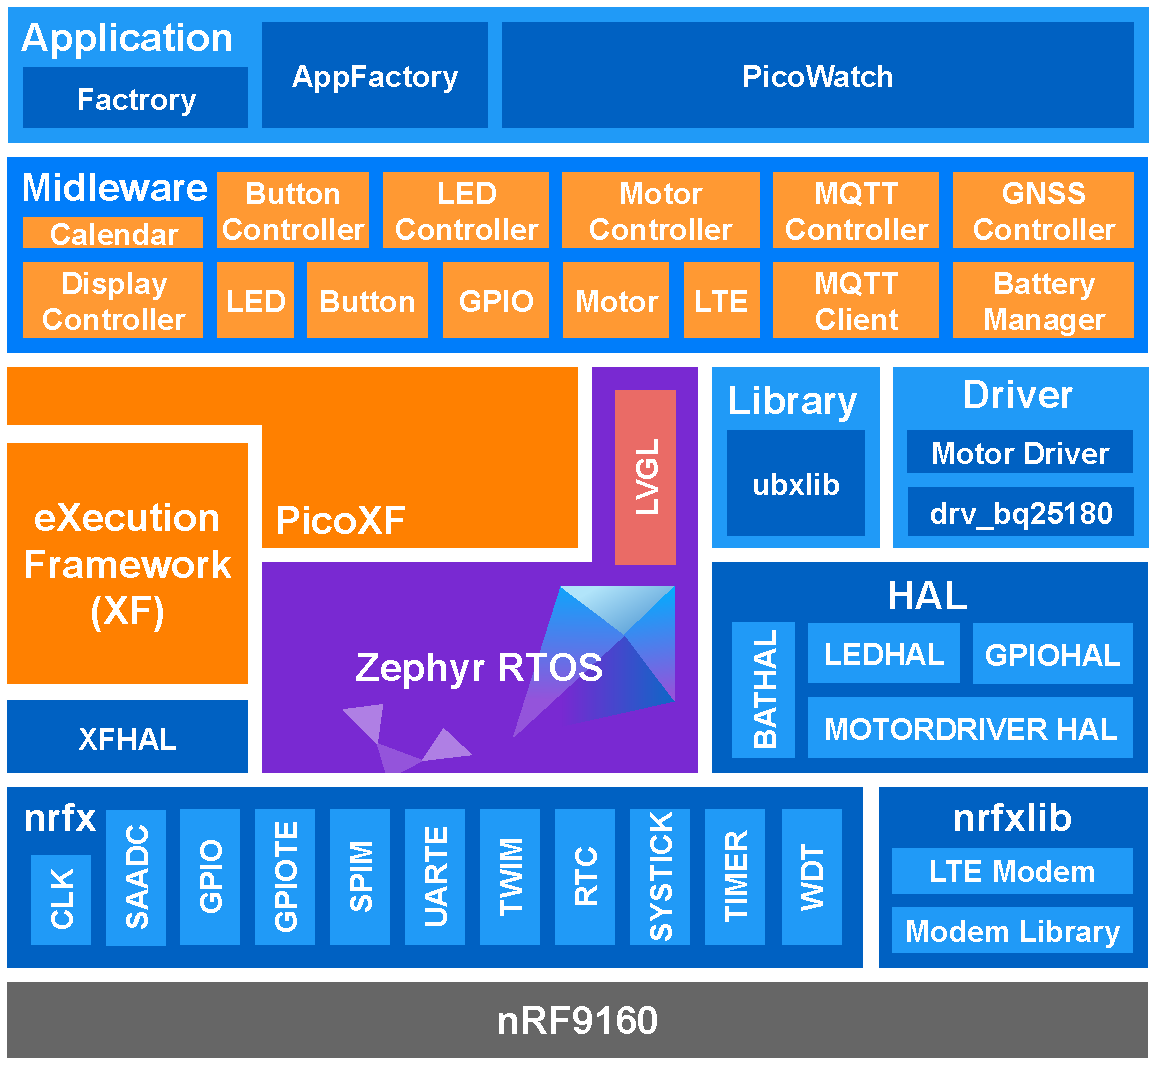
\includegraphics[width=0.75\textwidth]{Include/Figure/software/software_layers.pdf}
	\caption{\textit{LTEWatch} Software Architecture}
	\label{fig:software_layers}
\end{figure}

As shown in figure \ref{fig:software_layers}, the application requires the integration of many \textit{APIs} from the \textsc{Nordic Semiconductor} \textit{nrfx} driver set. These \textit{API} are either directly used by the \textit{LTEWatch} application, or required by the \textit{Zephyr} \textit{RTOS} which is the main component of the software.\\

The \textit{LTEWatch} firmware is an event-based application. This means that each process is triggered by events such as timeout triggered, \textit{GPIO} triggered or software triggered events. Since the application needs to be as responsive as possible, every submitted event needs to be stored, executed, and disposed of by an event manager unit, also known as an executive framework.\\

The \textit{Institute of Industrial System} of the \textit{HES-SO Wallis (HEVS)} has developed its own executive framework: \textbf{\textit{eXecution Framework}(\textit{XF})}. This \textit{XF} is used by the \textit{LTEWatch} firmware to implement an event-based application. Besides the integrated \textit{XF}, a more compact and simpler version of external framework \textit{PicoXF} is implemented for reasons that will be covered later.

\subsection{Introduction to \textit{nRF Connect SDK} from \textsc{Nordic Semi.}}

Before diving into the \textit{LTEWatch} firmware, it seems worth having a good understanding of the \textit{nRF Connect SDK} of \textsc{Nordic Semi}.\\

\textit{nRF Connect SDK} is an open-source and optimized cellular IoT (\textit{LTE-M}/\textit{NB-IoT}), \textit{Bluetooth Low Energy}, \textit{Thread}, \textit{Zigbee}, and \textit{Bluetooth mesh stacks} software development kit which includes the \textit{Zephyr} real-time operating system (\textit{RTOS}). The \textsc{nRF Connect SDK} enables to develop application for nRF52, nRF53, and nRF91 Series devices. The \textit{nRF Connect SDK} source code is fully accessible on \textsc{Nordic Semi.}'s \textit{"nrfconnect"} repository: \url{https://github.com/nrfconnect}.

\begin{flushleft}
The \textit{nRF Connect SDK} from \textsc{Nordic Semi.} contains the following modules:
\end{flushleft}
\begin{enumerate}
\item \textbf{sdk-nrf \textit{(nrfx)} : }Contains applications, samples, libraries, and drivers that are specifically targeted for Nordic Semiconductor devices.
\item \textbf{sdk-nrfxlib \textit{(nrfxlib)} :} Contains closed-source libraries and modules in binary format.
\item \textbf{sdk-zephyr \textit{(Zephyr RTOS)} :} Contains a fork of the \textit{Zephyr} project, which provides samples, libraries, and drivers for a wide variety of devices, including Nordic Semiconductor devices.
\item \textbf{sdk-mcuboot \textit{(mcuboot)}:} Contains a fork of the \textit{MCUboot} project, which provides a secure bootloader application. You can find the fork in \codeword{bootloader/mcuboot} after obtaining the \textsc{nRF Connect SDK} source code.
\end{enumerate}

\subsection{\textsc{Nordic Semi.} Driver Package (\textit{nrfx})}
\subsubsection{Overview:}
The replacement of the old \textit{"nRF5 SDK"} from \textsc{Nordic Semi.} with the new \textit{"nRF Connect SDK"} required to export all the drivers from their previous \textit{SDK} to ensure compatibility with previously developed applications, or at leas to facilitate as much as possible port to the new \textit{SDK}.\\

In the new \textit{nRF Connect SDK}, \textsc{Nordic Semi.}'s SoCs peripherals drivers are contained in \textit{nrfx}. \textsc{Nordic Semi.} also wanted to provide drivers that could be used in various environments without needing to integrate other parts of \textit{SDK}, if unnecessary, that's why they regrouped all drivers in \textit{nrfx}. \\

More detailed information about \textit{nrfx} is available on their online documentation: \url{https://developer.nordicsemi.com/nRF_Connect_SDK/doc/latest/nrfx/index.html}.

\pagebreak

\subsubsection{SoC Driver Compatibility Comparison Table:}
Before using any drivers or \textit{APis} from \textit{nrfx}, it is necessary to understand which drivers are supported by which SoC, in this case the \textit{nRF9160 SiP}.\\

The comparative overview of drivers compatibility of each SoCs from \textsc{Nordic Semi.} is presented in the following table \ref{tab:nrfx_driver_tab}:

\begin{table}[H]
\centering
\resizebox{\textwidth}{!}{\begin{tabular}{l|c|c|c|c|c|c|c|c|c}
\textbf{Driver} & \textbf{\textit{nRF}51xx} & \textbf{\textit{nRF}52805} & \textbf{\textit{nRF}5281x} & \textbf{\textit{nRF}52820} & \textbf{\textit{nRF}52832} & \textbf{\textit{nRF}52833} & \textbf{\textit{nRF}52840} & \textbf{\textit{nRF}5340} & \textcolor{blue}{\textbf{\textit{nRF}9160}} \\\hline
\textbf{AAR} & \textcolor{mygreen}{\cmark} & \textcolor{mygreen}{\cmark} & \textcolor{mygreen}{\cmark} &  \textcolor{mygreen}{\cmark} & \textcolor{mygreen}{\cmark} & \textcolor{mygreen}{\cmark} & \textcolor{mygreen}{\cmark} & \textcolor{mygreen}{\cmark} & \textcolor{red}{\xmark} \\
\textbf{ACL} & \textcolor{red}{\xmark} & \textcolor{red}{\xmark} & \textcolor{red}{\xmark} & \textcolor{mygreen}{\cmark} & \textcolor{red}{\xmark} & \textcolor{mygreen}{\cmark} & \textcolor{mygreen}{\cmark} & \textcolor{mygreen}{\cmark} & \textcolor{red}{\xmark} \\
\textbf{ADC} & \textcolor{mygreen}{\cmark} & \textcolor{red}{\xmark} & \textcolor{red}{\xmark} & \textcolor{red}{\xmark} & \textcolor{red}{\xmark} &  \textcolor{red}{\xmark} & \textcolor{red}{\xmark} & \textcolor{red}{\xmark} & \textcolor{red}{\xmark} \\
\textbf{BPROT} & \textcolor{red}{\xmark} &  \textcolor{mygreen}{\cmark} &  \textcolor{mygreen}{\cmark} &  \textcolor{red}{\xmark} &  \textcolor{mygreen}{\cmark} &   \textcolor{red}{\xmark} & \textcolor{red}{\xmark} &  \textcolor{red}{\xmark} & \textcolor{red}{\xmark} \\
\textbf{CACHE} & \textcolor{red}{\xmark} &  \textcolor{red}{\xmark} & \textcolor{red}{\xmark} & \textcolor{red}{\xmark} & \textcolor{red}{\xmark} &  \textcolor{red}{\xmark} &  \textcolor{red}{\xmark} &  \textcolor{mygreen}{\cmark} & \textcolor{red}{\xmark} \\
\textbf{CCM} &  \textcolor{mygreen}{\cmark} & \textcolor{mygreen}{\cmark} &  \textcolor{mygreen}{\cmark} &  \textcolor{mygreen}{\cmark} &  \textcolor{mygreen}{\cmark} &   \textcolor{mygreen}{\cmark} &  \textcolor{mygreen}{\cmark} &  \textcolor{mygreen}{\cmark} &  \textcolor{red}{\xmark} \\
\textbf{CLOCK} & \textcolor{mygreen}{\cmark} & \textcolor{mygreen}{\cmark} & \textcolor{mygreen}{\cmark} & \textcolor{mygreen}{\cmark} & \textcolor{mygreen}{\cmark} &  \textcolor{mygreen}{\cmark} & \textcolor{mygreen}{\cmark} & \textcolor{mygreen}{\cmark} & \textcolor{mygreen}{\cmark} \\
\textbf{COMP} & \textcolor{red}{\xmark} & \textcolor{red}{\xmark} & \textcolor{mygreen}{\cmark} &  \textcolor{mygreen}{\cmark} & \textcolor{mygreen}{\cmark} & \textcolor{mygreen}{\cmark} & \textcolor{mygreen}{\cmark} & \textcolor{mygreen}{\cmark} & \textcolor{red}{\xmark} \\
\textbf{DCNF} &\textcolor{red}{\xmark} &\textcolor{red}{\xmark} &\textcolor{red}{\xmark} &\textcolor{red}{\xmark} &\textcolor{red}{\xmark} &\textcolor{red}{\xmark} &\textcolor{red}{\xmark} &\textcolor{mygreen}{\cmark} &\textcolor{red}{\xmark} \\
\textbf{DPPI} &\textcolor{red}{\xmark} &\textcolor{red}{\xmark} &\textcolor{red}{\xmark} &\textcolor{red}{\xmark} &\textcolor{red}{\xmark} &\textcolor{red}{\xmark} &\textcolor{red}{\xmark} &\textcolor{mygreen}{\cmark} &\textcolor{mygreen}{\cmark} \\
\textbf{ECB} &\textcolor{mygreen}{\cmark} &\textcolor{mygreen}{\cmark} &\textcolor{mygreen}{\cmark} &\textcolor{mygreen}{\cmark} &\textcolor{mygreen}{\cmark} &\textcolor{mygreen}{\cmark} &\textcolor{mygreen}{\cmark} &\textcolor{mygreen}{\cmark} &\textcolor{red}{\xmark} \\
\textbf{EGU} & \textcolor{red}{\xmark} & \textcolor{mygreen}{\cmark} & \textcolor{mygreen}{\cmark} & \textcolor{mygreen}{\cmark} & \textcolor{mygreen}{\cmark} & \textcolor{mygreen}{\cmark} & \textcolor{mygreen}{\cmark} & \textcolor{mygreen}{\cmark} & \textcolor{mygreen}{\cmark} \\
\textbf{FICR} &\textcolor{mygreen}{\cmark} &\textcolor{mygreen}{\cmark} &\textcolor{mygreen}{\cmark} &\textcolor{mygreen}{\cmark} &\textcolor{mygreen}{\cmark} &\textcolor{mygreen}{\cmark} &\textcolor{mygreen}{\cmark} &\textcolor{mygreen}{\cmark} &\textcolor{mygreen}{\cmark} \\
\textbf{FPU} & \textcolor{red}{\xmark} &\textcolor{red}{\xmark} &\textcolor{red}{\xmark} &\textcolor{red}{\xmark} &\textcolor{red}{\xmark} &\textcolor{red}{\xmark} &\textcolor{red}{\xmark} &\textcolor{mygreen}{\cmark} &\textcolor{red}{\xmark} \\
\textbf{GPIO} & \textcolor{mygreen}{\cmark} &\textcolor{mygreen}{\cmark} &\textcolor{mygreen}{\cmark} &\textcolor{mygreen}{\cmark} &\textcolor{mygreen}{\cmark} &\textcolor{mygreen}{\cmark} &\textcolor{mygreen}{\cmark} &\textcolor{mygreen}{\cmark} &\textcolor{mygreen}{\cmark} \\
\textbf{GPIOTE} &\textcolor{mygreen}{\cmark} &\textcolor{mygreen}{\cmark} &\textcolor{mygreen}{\cmark} &\textcolor{mygreen}{\cmark} &\textcolor{mygreen}{\cmark} &\textcolor{mygreen}{\cmark} &\textcolor{mygreen}{\cmark} &\textcolor{mygreen}{\cmark} &\textcolor{mygreen}{\cmark} \\
\textbf{I2S} &\textcolor{red}{\xmark} &\textcolor{red}{\xmark} &\textcolor{red}{\xmark} &\textcolor{red}{\xmark} &\textcolor{mygreen}{\cmark} &\textcolor{mygreen}{\cmark} &\textcolor{mygreen}{\cmark} &\textcolor{mygreen}{\cmark} &\textcolor{mygreen}{\cmark} \\
\textbf{IPC} &\textcolor{red}{\xmark} &\textcolor{red}{\xmark} &\textcolor{red}{\xmark} &\textcolor{red}{\xmark} &\textcolor{red}{\xmark} &\textcolor{red}{\xmark} &\textcolor{red}{\xmark} &\textcolor{mygreen}{\cmark} &\textcolor{mygreen}{\cmark} \\
\textbf{KMU} &\textcolor{red}{\xmark} &\textcolor{red}{\xmark} &\textcolor{red}{\xmark} &\textcolor{red}{\xmark} &\textcolor{red}{\xmark} &\textcolor{red}{\xmark} &\textcolor{red}{\xmark} &\textcolor{mygreen}{\cmark} &\textcolor{mygreen}{\cmark} \\
\textbf{LPCOMP} &\textcolor{mygreen}{\cmark} &\textcolor{red}{\xmark} &\textcolor{red}{\xmark} &\textcolor{red}{\xmark} &\textcolor{mygreen}{\cmark} &\textcolor{mygreen}{\cmark} &\textcolor{mygreen}{\cmark} &\textcolor{mygreen}{\cmark} &\textcolor{red}{\xmark} \\
\textbf{MPU} &\textcolor{mygreen}{\cmark} &\textcolor{red}{\xmark} &\textcolor{red}{\xmark} &\textcolor{red}{\xmark} &\textcolor{red}{\xmark} &\textcolor{red}{\xmark} &\textcolor{red}{\xmark} &\textcolor{red}{\xmark} &\textcolor{red}{\xmark} \\
\textbf{MUTEX} &\textcolor{red}{\xmark} &\textcolor{red}{\xmark} &\textcolor{red}{\xmark} &\textcolor{red}{\xmark} &\textcolor{red}{\xmark} &\textcolor{red}{\xmark} &\textcolor{red}{\xmark} &\textcolor{mygreen}{\cmark} &\textcolor{red}{\xmark} \\
\textbf{MWU} &\textcolor{red}{\xmark} &\textcolor{red}{\xmark} &\textcolor{red}{\xmark} &\textcolor{red}{\xmark} &\textcolor{mygreen}{\cmark} &\textcolor{mygreen}{\cmark} &\textcolor{mygreen}{\cmark} &\textcolor{red}{\xmark} &\textcolor{red}{\xmark} \\
\textbf{NFCT} &\textcolor{red}{\xmark} &\textcolor{red}{\xmark} &\textcolor{red}{\xmark} &\textcolor{red}{\xmark} &\textcolor{mygreen}{\cmark} &\textcolor{mygreen}{\cmark} &\textcolor{mygreen}{\cmark} &\textcolor{mygreen}{\cmark} &\textcolor{red}{\xmark} \\
\textbf{NVMC} &\textcolor{mygreen}{\cmark} &\textcolor{mygreen}{\cmark} &\textcolor{mygreen}{\cmark} &\textcolor{mygreen}{\cmark} &\textcolor{mygreen}{\cmark} &\textcolor{mygreen}{\cmark} &\textcolor{mygreen}{\cmark} &\textcolor{mygreen}{\cmark} &\textcolor{mygreen}{\cmark} \\
\textbf{PDM} &\textcolor{red}{\xmark} &\textcolor{red}{\xmark} &\textcolor{mygreen}{\cmark} &\textcolor{red}{\xmark} &\textcolor{mygreen}{\cmark} &\textcolor{mygreen}{\cmark} &\textcolor{mygreen}{\cmark} &\textcolor{mygreen}{\cmark} &\textcolor{mygreen}{\cmark} \\
\textbf{POWER} &\textcolor{mygreen}{\cmark} &\textcolor{mygreen}{\cmark} &\textcolor{mygreen}{\cmark} &\textcolor{mygreen}{\cmark} &\textcolor{mygreen}{\cmark} &\textcolor{mygreen}{\cmark} &\textcolor{mygreen}{\cmark} &\textcolor{mygreen}{\cmark} &\textcolor{mygreen}{\cmark} \\
\textbf{PPI} &\textcolor{mygreen}{\cmark} &\textcolor{mygreen}{\cmark} &\textcolor{mygreen}{\cmark} &\textcolor{mygreen}{\cmark} &\textcolor{mygreen}{\cmark} &\textcolor{mygreen}{\cmark} &\textcolor{mygreen}{\cmark} &\textcolor{red}{\xmark} &\textcolor{red}{\xmark} \\
\textbf{PWM} &\textcolor{red}{\xmark} &\textcolor{red}{\xmark} &\textcolor{mygreen}{\cmark} &\textcolor{red}{\xmark} &\textcolor{mygreen}{\cmark} &\textcolor{mygreen}{\cmark} &\textcolor{mygreen}{\cmark} &\textcolor{mygreen}{\cmark} &\textcolor{mygreen}{\cmark} \\
\textbf{QDEC} &\textcolor{mygreen}{\cmark} &\textcolor{mygreen}{\cmark} &\textcolor{mygreen}{\cmark} &\textcolor{mygreen}{\cmark} &\textcolor{mygreen}{\cmark} &\textcolor{mygreen}{\cmark} &\textcolor{mygreen}{\cmark} &\textcolor{mygreen}{\cmark} &\textcolor{red}{\xmark} \\
\textbf{QSPI} &\textcolor{red}{\xmark} &\textcolor{red}{\xmark} &\textcolor{red}{\xmark} &\textcolor{red}{\xmark} &\textcolor{red}{\xmark} &\textcolor{red}{\xmark} &\textcolor{mygreen}{\cmark} &\textcolor{mygreen}{\cmark} &\textcolor{red}{\xmark} \\
\textbf{RADIO} &\textcolor{mygreen}{\cmark} &\textcolor{mygreen}{\cmark} &\textcolor{mygreen}{\cmark} &\textcolor{mygreen}{\cmark} &\textcolor{mygreen}{\cmark} &\textcolor{mygreen}{\cmark} &\textcolor{mygreen}{\cmark} &\textcolor{mygreen}{\cmark} &\textcolor{red}{\xmark} \\
\textbf{RNG} &\textcolor{mygreen}{\cmark} &\textcolor{mygreen}{\cmark} &\textcolor{mygreen}{\cmark} &\textcolor{mygreen}{\cmark} &\textcolor{mygreen}{\cmark} &\textcolor{mygreen}{\cmark} &\textcolor{mygreen}{\cmark} &\textcolor{mygreen}{\cmark} &\textcolor{red}{\xmark} \\
\textbf{RTC} &\textcolor{mygreen}{\cmark} &\textcolor{mygreen}{\cmark} &\textcolor{mygreen}{\cmark} &\textcolor{mygreen}{\cmark} &\textcolor{mygreen}{\cmark} &\textcolor{mygreen}{\cmark} &\textcolor{mygreen}{\cmark} &\textcolor{mygreen}{\cmark} &\textcolor{mygreen}{\cmark} \\
\textbf{SAADC} &\textcolor{red}{\xmark} &\textcolor{mygreen}{\cmark} &\textcolor{mygreen}{\cmark} &\textcolor{red}{\xmark} &\textcolor{mygreen}{\cmark} &\textcolor{mygreen}{\cmark} &\textcolor{mygreen}{\cmark} &\textcolor{mygreen}{\cmark} &\textcolor{mygreen}{\cmark} \\
\textbf{SPI} &\textcolor{mygreen}{\cmark} &\textcolor{mygreen}{\cmark} &\textcolor{mygreen}{\cmark} &\textcolor{mygreen}{\cmark} &\textcolor{mygreen}{\cmark} &\textcolor{mygreen}{\cmark} &\textcolor{mygreen}{\cmark} &\textcolor{red}{\xmark} &\textcolor{red}{\xmark} \\
\textbf{SPIM} &\textcolor{red}{\xmark} &\textcolor{mygreen}{\cmark} &\textcolor{mygreen}{\cmark} &\textcolor{mygreen}{\cmark} &\textcolor{mygreen}{\cmark} &\textcolor{mygreen}{\cmark} &\textcolor{mygreen}{\cmark} &\textcolor{mygreen}{\cmark} &\textcolor{mygreen}{\cmark} \\
\textbf{SPIS} &\textcolor{mygreen}{\cmark} &\textcolor{mygreen}{\cmark} &\textcolor{mygreen}{\cmark} &\textcolor{mygreen}{\cmark} &\textcolor{mygreen}{\cmark} &\textcolor{mygreen}{\cmark} &\textcolor{mygreen}{\cmark} &\textcolor{mygreen}{\cmark} &\textcolor{mygreen}{\cmark} \\
\textbf{SPU} &\textcolor{red}{\xmark} &\textcolor{red}{\xmark} &\textcolor{red}{\xmark} &\textcolor{red}{\xmark} &\textcolor{red}{\xmark} &\textcolor{red}{\xmark} &\textcolor{red}{\xmark} &\textcolor{mygreen}{\cmark} &\textcolor{mygreen}{\cmark} \\
\textbf{SYSTICK} & \textcolor{red}{\xmark} & \textcolor{mygreen}{\cmark} & \textcolor{mygreen}{\cmark} & \textcolor{mygreen}{\cmark} & \textcolor{mygreen}{\cmark} & \textcolor{mygreen}{\cmark} & \textcolor{mygreen}{\cmark} & \textcolor{mygreen}{\cmark} & \textcolor{mygreen}{\cmark} \\
\textbf{TEMP} &\textcolor{mygreen}{\cmark} &\textcolor{mygreen}{\cmark} &\textcolor{mygreen}{\cmark} &\textcolor{mygreen}{\cmark} &\textcolor{mygreen}{\cmark} &\textcolor{mygreen}{\cmark} &\textcolor{mygreen}{\cmark} &\textcolor{mygreen}{\cmark} &\textcolor{red}{\xmark} \\
\textbf{TIMER} &\textcolor{mygreen}{\cmark} &\textcolor{mygreen}{\cmark} &\textcolor{mygreen}{\cmark} &\textcolor{mygreen}{\cmark} &\textcolor{mygreen}{\cmark} &\textcolor{mygreen}{\cmark} &\textcolor{mygreen}{\cmark} &\textcolor{mygreen}{\cmark} &\textcolor{mygreen}{\cmark} \\
\textbf{TWI} &\textcolor{mygreen}{\cmark} &\textcolor{mygreen}{\cmark} &\textcolor{mygreen}{\cmark} &\textcolor{mygreen}{\cmark} &\textcolor{mygreen}{\cmark} &\textcolor{mygreen}{\cmark} &\textcolor{mygreen}{\cmark} &\textcolor{red}{\xmark} &\textcolor{red}{\xmark} \\
\textbf{TWIM} &\textcolor{red}{\xmark} &\textcolor{mygreen}{\cmark} &\textcolor{mygreen}{\cmark} &\textcolor{mygreen}{\cmark} &\textcolor{mygreen}{\cmark} &\textcolor{mygreen}{\cmark} &\textcolor{mygreen}{\cmark} &\textcolor{mygreen}{\cmark} &\textcolor{mygreen}{\cmark} \\
\textbf{TWIS} &\textcolor{red}{\xmark} &\textcolor{mygreen}{\cmark} &\textcolor{mygreen}{\cmark} &\textcolor{mygreen}{\cmark} &\textcolor{mygreen}{\cmark} &\textcolor{mygreen}{\cmark} &\textcolor{mygreen}{\cmark} &\textcolor{mygreen}{\cmark} &\textcolor{mygreen}{\cmark} \\
\textbf{UART} &\textcolor{mygreen}{\cmark} &\textcolor{mygreen}{\cmark} &\textcolor{mygreen}{\cmark} &\textcolor{mygreen}{\cmark} &\textcolor{mygreen}{\cmark} &\textcolor{mygreen}{\cmark} &\textcolor{mygreen}{\cmark} &\textcolor{red}{\xmark} &\textcolor{red}{\xmark} \\
\textbf{UARTE} &\textcolor{red}{\xmark} &\textcolor{mygreen}{\cmark} &\textcolor{mygreen}{\cmark} &\textcolor{mygreen}{\cmark} &\textcolor{mygreen}{\cmark} &\textcolor{mygreen}{\cmark} &\textcolor{mygreen}{\cmark} &\textcolor{mygreen}{\cmark} &\textcolor{mygreen}{\cmark} \\
\textbf{USBD} &\textcolor{red}{\xmark} &\textcolor{red}{\xmark} &\textcolor{red}{\xmark} &\textcolor{mygreen}{\cmark} &\textcolor{red}{\xmark} &\textcolor{mygreen}{\cmark} &\textcolor{mygreen}{\cmark} &\textcolor{mygreen}{\cmark} &\textcolor{red}{\xmark} \\
\textbf{VMC} &\textcolor{red}{\xmark} &\textcolor{red}{\xmark} &\textcolor{red}{\xmark} &\textcolor{red}{\xmark} &\textcolor{red}{\xmark} &\textcolor{red}{\xmark} &\textcolor{red}{\xmark} &\textcolor{mygreen}{\cmark} &\textcolor{mygreen}{\cmark} \\
\textbf{WDT} &\textcolor{mygreen}{\cmark} &\textcolor{mygreen}{\cmark} &\textcolor{mygreen}{\cmark} &\textcolor{mygreen}{\cmark} &\textcolor{mygreen}{\cmark} &\textcolor{mygreen}{\cmark} &\textcolor{mygreen}{\cmark} &\textcolor{mygreen}{\cmark} &\textcolor{mygreen}{\cmark}
\end{tabular}}
\caption{SoC Driver Compatibility Comparison Table - Source:\cite{nrfx}}
\label{tab:nrfx_driver_tab}
\end{table}

\textit{LTEWatch} application require several drivers that are listed in table \ref{tab:nrfx_driver_tab}. Using the list of supported drivers for the \textit{nRF9160} SoC and the function block decomposition it is possible to list all necessary drivers required for \textit{LTEWatch} application using \textit{nRF9160} SoC.\\

\pagebreak

\begin{flushleft}
 The list of drivers required by the \textit{LTEWatch} application is the following:
\end{flushleft}
 
\begin{enumerate}
\item \textbf{Buttons, LEDs and other DI/O:}
\begin{itemize}
\item GPIO: \textit{Hardware access layer} for managing the GPIO peripheral
\item GPIOTE: \textit{GPIO Task Event} peripheral driver
\end{itemize}

\item \textbf{Display \& Accelerometer:}
\begin{itemize}
\item SPIM: \textit{Serial Peripheral Interface Master} with \textit{EasyDMA} driver
\item SPIS: \textit{Serial Peripheral Interface Slave} with \textit{EasyDMA} driver
\end{itemize}

\item \textbf{Motors:}
\begin{itemize}
\item RTC: \textit{Real Timer Counter} peripheral driver
\end{itemize}

\item \textbf{Battery Manager \& \textit{GNSS} Controller:}
\begin{itemize}
\item SAADC: \textit{Successive Approximation ADC} peripheral driver
\item TWIM: \textit{Two Wire Interface Master} with \textit{EasyDMA} peripheral driver
\item TWIS: \textit{Two Wire Interface Slave} with \textit{EasyDMA} peripheral driver
\end{itemize}

\item \textbf{Debug \& Logging}
\begin{itemize}
\item UARTE: \textit{UART Task Event} peripheral driver
\end{itemize}

\item \textbf{Events, Timers and Timeouts Based Application:}
\begin{itemize}
\item CLOCK: Clock peripheral driver
\item SYSTICK: ARM(R) driver to configure \textit{SysTick} as a free-running timer used to generate delays and pool for short timeouts ($\leq$ \SI{250}{\micro\second})
\item TIMER: \textit{Timer} peripheral driver
\end{itemize}

\item \textbf{LTE Modem:}
\begin{itemize}
\item PDM: \textit{Pulse Density Modulation} peripheral driver
\end{itemize}

\item \textbf{Zephyr RTOS:}
\begin{itemize}
\item DPPI: \textit{Distributed Programmable Peripheral Interconnect} allocator
\item EGU: \textit{Event Generator Unit} peripheral driver
\item FICR: \textit{HAL} to get \textit{Factory Information Configuration Registers}
\item IPC: \textit{Interprocessor Communication} peripheral driver.
\item KMU: \textit{HAL} for managing the \textit{Key Management Unit} peripheral
\item NVMC: \textit{Non-Volatile Memory Controller} peripheral driver
\item POWER: Set of drivers for managing POWER peripherals
\item SPU: \textit{HAL} for managing the \textit{System Protection Unit} peripheral.
\item VMC: \textit{HAL} for managing the \textit{Volatile Memory Controller} peripheral
\item WDT: \textit{Watchdog Timer} peripheral driver
\end{itemize}
\end{enumerate}

\pagebreak

\subsection{\textit{Zephyr} Real Time Operating System (\textit{RTOS})}

\textit{Zephyr RTOS} is an open-source real time operating system with a small-footprint that is specially designed for resource constrained and embedded applications. Compact embedded portable applications such as simple environmental sensors and LED oriented wearables but also more complex and sophisticated portable applications, like smart-watches, embedded controllers and \textit{IoT} wireless applications.

\subsection{\textsc{Nordic Semi.} Libraries \& Modules (\textit{nrfxlib})}

As described on \textsc{Nordic Semi.}'s online documentation\cite{nrfxlib}, \textit{nrfxlib} contains \textit{RTOS}-independent libraries and modules for \textsc{Nordic Semi.} SoCs such as the \textit{Modem Library} that is required by the \textit{LTEWatch} firmware to implement \textit{LTE-M/NB-IoT} and \textit{MQTT} applications.

\subsubsection{\textit{nrfxlib} Modem library:}

The \textit{Modem Library} is an interface provided by \textsc{Nordic Semi.} that is used for:
\begin{itemize}
\item operating the \textit{nRF9160} modem,
\item establishing the \textit{LTE-M} and \textit{NB-IoT} connections,
\item and receiving the position data (GPS).
\end{itemize}

In the case of the \textit{LTEWatch} application, this library is used to operate the \textit{nRF9160} modem and to establish the \textit{LTE-M/NB-IoT} connections. Features relatives to \textit{GNSS} is not requiered because \textit{LTEWatch} uses an external \textit{GNSS} receiver that only necessitates to implement a serial \textit{I2C} bus communication to configure the receiver and to get position data.

\section{External Library}
The \textit{LTEWatch} application implement a display and an external \textit{GNSS} receiver. Both modules requires drivers and libraries to be reconfigured and operated.
\begin{flushleft}
The application implement the two following external libraries:
\end{flushleft}
\begin{enumerate}
\item \textbf{LVGL}: An open-source, graphics library that is already integrated in \textit{Zephyr}
\item \textbf{ubxlib}: An open-source library for \textsc{u-blox} products and services
\end{enumerate}

\subsection{Light and Versatile Graphics Library (\textit{LVGL})}
\subsubsection{\textit{LVGL} Overview (source:\cite{lvgl_lib}):}
\textit{LVGL} is very popular, free and open-source embedded graphics library compatible with any \textit{MCU}, \textit{MPU}, and display type that is supported by many vendors and project such as Arm, STM32, NXP, Espressif, Nuvoton, Arduino, RT-Thread, Zephyr, NuttX, Adafruit and many more.\\

The \textit{LVGL} library provides all necessary features to create all king of \textit{GUIs} with over 30 built-in widgets, style system, web inspired layout manager, typography system supporting many languages.
\begin{flushleft}
 The library implementation only requires the following specifications:
\end{flushleft}
\begin{enumerate}
\item \SI{32}{\kilo\byte} of \textit{RAM}
\item \SI{128}{\kilo\byte} of \textit{Flash}
\item A \textit{C} compiler
\item A frame buffer
\item At least an $1/10$ screen sized buffer for rendering
\end{enumerate}

\subsubsection{\textit{LVGL} Features:}
\begin{flushleft}
The \textit{LVGL} library provides the following interesting features (src.\cite{lvgl_lib}):
\end{flushleft}

\begin{itemize}
\item \textbf{Free and Portable:}
\begin{itemize}
\item A fully portable C (C++ compatible) library with no external dependencies.
\item Can be compiled to any MCU or MPU, with any (RT)OS.
\item Supports monochrome, ePaper, OLED or TFT displays, or even monitors. Porting Guide
\item Distributed under the MIT licence, so you can easily use it in commercial projects too.
\item Needs only \SI{32}{\kilo\byte} \textit{RAM} and \SI{128}{\kilo\byte} \textit{Flash}, a frame buffer, and at least an $1/10$ screen sized buffer for rendering.
\item OS, External memory and \textit{GPU} are supported but not required.
\end{itemize}
\item \textbf{Widgets, Styles, Layouts and more:}
\begin{itemize}
\item 30+ built-in Widgets:  Button, Label, Slider, Chart, Keyboard, Meter, Arc, Table and many more.
\item Flexible Style system with $\approx 100$ style properties to customize any part of the widgets in any state.
\item \textit{Flexbox} and \textit{Grid}-like layouts engines to automatically size and position the widgets in a responsive way.
\item Texts are rendered with \textit{UTF-8} encoding supporting CJK, Thai, Hindi, Arabic, Persian writing systems.
\item Word wrapping, kerning, text scrolling, sub-pixel rendering, Pinyin-IME Chinese input, Emojis in texts.
\item Rendering engine supporting animations, anti-aliasing, opacity, smooth scrolling, shadows, image transformation, etc  
\item Supports Mouse, Touchpad, Keypad, Keyboard, External buttons, Encoder Input devices.
\item Multiple display support.
\end{itemize}
\end{itemize}

\subsubsection{\textit{LVGL} Installation and Integration Process:}
The \textit{LVGL} library is directly integrated in the \textit{Zephyr RTOS}, which makes its implementation fairly easy.\\

The installation and integration process is as follow:
\begin{enumerate}
\item In the application configuration file (\textit{Kconfig}):
\begin{enumerate}
\item Enable \textit{Zephyr} display driver and library with: \codeword{CONFIG_DISPLAY=y}
\item Enable the \textit{LVGL} library with: \codeword{CONFIG_LVGL=y}
\item If required, it is possible to configure custom memory for the \textit{LVGL} with:
\begin{itemize}
\item \codeword{CONFIG_LV_MEM_CUSTOM=y}
\item \codeword{CONFIG_LV_Z_MEM_POOL_NUMBER_BLOCKS=16}
\end{itemize}
\item Enable the driver for \textit{SHARP MIP LCD LS0XX} with:
\begin{itemize}
\item \codeword{CONFIG_LS0XX=y}
\end{itemize}
\item If required, configure \textit{LVGL} specific proprieties:
\begin{itemize}
\item Enable \textit{label} type widget: \codeword{CONFIG_LV_USE_LABEL=y}
\item Enable \textit{image} type widget: \codeword{CONFIG_LV_USE_IMG=y}
\item Set display color depth: \codeword{CONFIG_LV_COLOR_DEPTH_1=y}
\item Set text font style and size: \\ \codeword{CONFIG_LV_FONT_DEFAULT_MONTSERRAT_16=y}
\item Set text format: \codeword{CONFIG_LV_TXT_ENC_UTF8=y}\\
\end{itemize}
\end{enumerate}
\item In the application \textit{Devicetree} overlay:
\begin{enumerate}
\item Enable the \textit{SHARP MIP LCD LS0XX} driver binding with:
\begin{lstlisting}[style=console]
chosen {
		zephyr,display = &ls0xx;
	};
\end{lstlisting}
\end{enumerate}
\item Include \codeword{lvgl.h} in each \textit{C/C++} application file that uses \textit{LVGL} library
\end{enumerate}

More detailed information about \textit{LVGL} library configuration and implementation is available on \textit{LVGL} online documentation: \url{https://docs.lvgl.io/master/index.html}.

\pagebreak

\subsection{\textsc{u-blox} Host Library (\textit{ubxlib})}
\subsubsection{\textit{ubxlib} Overview:}

The following description is sourced from the \textit{ubxlib} GitHub repository\cite{ubx_lib}.\\

The \textit{ubxlib} contains add-on for building embedded applications with u-blox products and services on \textit{MCU} and \textit{RTOS} \textit{SDKs}. The \textit{ubxlib} repository provides portable \textit{C} libraries APIs and many examples and sample code for an easier implementation process.\\


The \textit{ubxlib} library main features are:
\begin{itemize}
\item Supports the following \textsc{u-blox} modules:
\begin{itemize}
\item Cellular modules (\textit{2G/3G/4G})
\item Short-range modules (\textit{Bluetooth} and \textit{Wifi})
\item \textit{GNSS} positioning modules
\end{itemize}
\item Provides high level \textit{C} \textit{APIs} for customer applications such as connection to a network, \textit{TCP} socket opening, location establishment, and many others)
\item Compatibility with \textit{ARM} \textit{MCUs} and \textit{Zephyr} project
\end{itemize}

\begin{flushleft}
Figure \ref{fig:ubxlib_high_level} illustrates the \textit{ubxlib} library integration diagram:
\end{flushleft}
\begin{figure}[H]
	\centering
	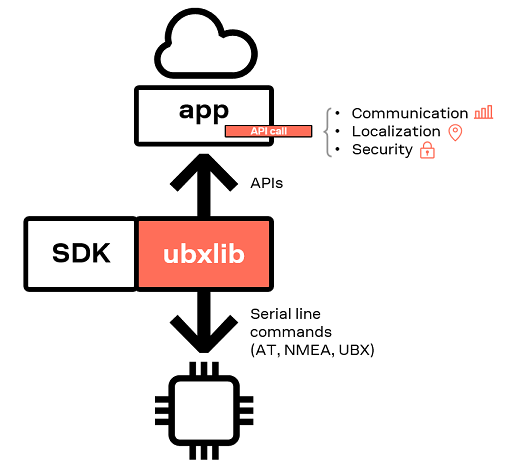
\includegraphics[width=0.6\textwidth]{Include/Figure/software/ubxlib_high_level.png}
	\caption{\textit{ubxlib} Library Integration Diagram - Source:\cite{ubx_lib}}
	\label{fig:ubxlib_high_level}
\end{figure}

\pagebreak

\subsubsection{Description of \textit{ubxlib} \textit{APIs}}

The \textit{ubxlib} repository\cite{ubx_lib} provides a visual illustration of the different \textit{APIs} contained in the library as well as their relationships with each other. This diagram is illustrated in figure \ref{fig:ubxlib_high_level}:

\begin{figure}[H]
	\centering
	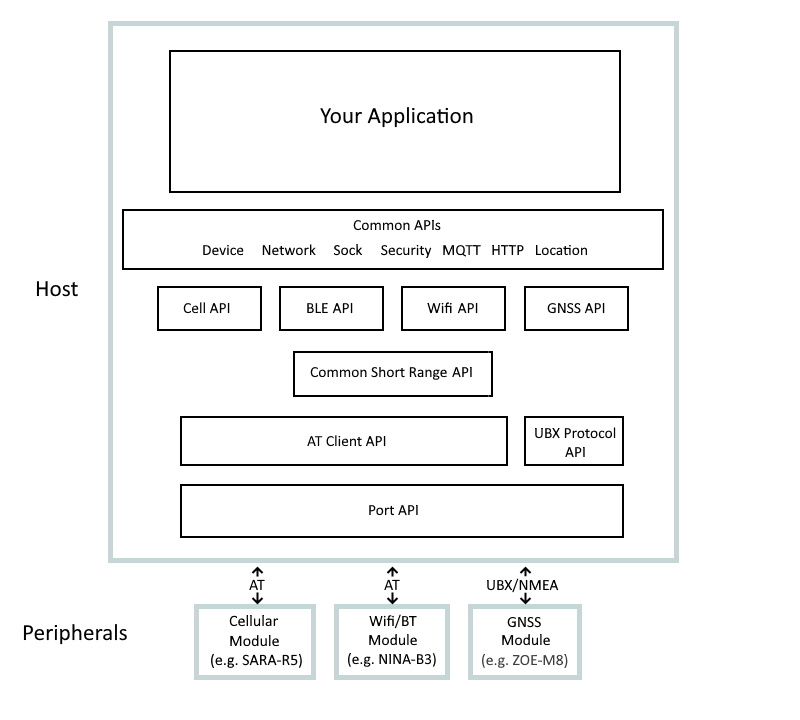
\includegraphics[width=0.8\textwidth]{Include/Figure/software/apis.jpg}
	\caption{\textit{ubxlib} Library \textit{APIs} Diagram - Source:\cite{ubx_lib}}
	\label{fig:ubxlib_high_level}
\end{figure}

The \textit{ubxlib} repository\cite{ubx_lib} also gives information about which \textit{APIs} to use for which application. The \textit{ubxlib} library usage recommendations are the following(src.\cite{ubx_lib}):

\begin{itemize}
\item \textit{Common Device} and \textit{network} \textit{APIs}: Used to quickly bring up a device/network such as \textit{cellular}, \textit{BLE/Wifi} or \textit{GNSS}
\item \textit{Common Sock API}: Used for application requiring a socket over the network
\item \textit{Common Security API}: Used for network that require security functionality
\item \textit{Common MQTT (mqtt\_client) API}: Used for \textit{MQTT} applications
\item \textit{Common HTTP (http\_client) API}: Used for HTTP applications
\item \textit{Common Location API}: Used for application requiring location fixes
\item \textit{Cell, Ble, Wifi, GNSS APIs}: Used for finer control and configuration
\item \textit{GNSS API}: Used for application requiring a specific \textit{GNSS} configuration
\item \textit{Common Short Range API}: Used for short range applications (\textit{BLE} or \textit{Wifi})
\item \textit{AT Client API}: Used by \textit{Cell} and \textit{Short Range APIs} to talk to AT-based u-blox modules
\item \textit{Port API}: Permits all of the above \textit{APIs} to run on different hosts
\end{itemize}

\subsubsection{Installation and Integration Process:}
The \textit{ubxlib} library is not integrated in \textit{Zephyr} project or \textit{nRF Connect SDK}, which imply, that the library must be linked to the application using the project \textit{CMake} linker file.\\

The installation and integration process of \textit{ubxlib} library is as follow:
\begin{enumerate}
\item Clone the \textit{ubxlib} GitHub repository in your local computer either in your \textit{Zephyr} root directory or either on a custom location with the shortest path possible: \url{https://github.com/u-blox/ubxlib}
\item In the application linker file \textit{CMakeLists.txt}:
\begin{enumerate}
\item Add the library to your project as an external module of \textit{Zephyr} using the \codeword{list(APPEND ZEPHYR_EXTRA_MODULES ...)} command:
\begin{lstlisting}[style=console]
list(APPEND ZEPHYR_EXTRA_MODULES "${<my_ubxlib_repo_path>/ubxlib")
\end{lstlisting}
\end{enumerate}
\item In the application configuration file (\textit{Kconfig}):
\begin{enumerate}
\item Enable the \textit{ubxlib} library with: \codeword{CONFIG_UBXLIB=y}
\end{enumerate}
\item For the \textit{LTEWatch} application, the following additional configuration is necessary:
\begin{enumerate}
\item Enable \textit{ubxlib }\textit{GNSS API}: \codeword{CONFIG_UBXLIB_GNSS=y}
\item Enable \textit{ubxlib }\textit{Cell API} (not used but is required by \textit{GNSS API} dependencies): \codeword{CONFIG_UBXLIB_CELL=y}
\item Disable \textit{Test API} to reduce extra module size: \codeword{CONFIG_UBXLIB_TEST=n}
\end{enumerate}
\item Include necessary \textit{ubxlib} header files in each \textit{C/C++} application files that use \textsc{u-blox} modules or \textit{APIs}
\end{enumerate}

\pagebreak

\section{\textit{LTEWatch} Hardware Description}

Once the firmware is decomposed in functional block and before looking at the application software, it is necessary to clearly defines the target device hardware, the application configuration and the project management file.\\

This section covers hardware description process in \textit{Zephyr} environment, starting by  system hardware description and configuration using \textit{Devicetree}, project source files management and external library integration using \textit{CMakeLists.txt} and finally application configuration using \textit{Kconfig} file (\textit{conf.prj}).


\subsection{Pin Assignment of \textit{LTEWatch} Prototype Board}
The table \ref{tab:gpio_ltewatch_board} describes the pin assignment of the \textit{LTEWatch} prototype board:

\begin{table}[H]
\centering
\resizebox{\textwidth}{!}{\begin{tabular}{l c c l l}
\textbf{PIN} & \textbf{I/O} & \textbf{CFG} & \textbf{SIGNAL} & \textbf{DESCRIPTION}\\\hline \hline
P0.00  & DO\footnote{\textit{DO}: Digital Output} & - & M8 & Stepper Motor driving output\textit{D3M4}\\
P0.01  & DO & - & M7 & Stepper Motor driving output\textit{D3COM}\\
P0.02  & DO & - & M6 & Stepper Motor driving output\textit{D3M1}\\
P0.03  & DO & - & M5 & Stepper Motor driving output\textit{D2M4}\\
P0.04  & DO & - & M4 & Stepper Motor driving output\textit{D2MCOM}\\
P0.05  & DO & - & M3 & Stepper Motor driving output\textit{D2M1}\\
P0.06  & SO\footnote{\textit{SO}: Serial Output} & UART & USB\_TX & \textit{TX} signal of the \textit{USB-to-UART} interface\\
P0.07  & SI\footnote{\textit{SI}: Serial Input} & UART & USB\_RX & \textit{RX} signal of the \textit{USB-to-UART} interface\\
P0.08  & SIO & I2C & SDA & Data line of \textit{I2C} Bus\\
P0.09  & CLK & I2C & SCL & Clock line of \textit{I2C} Bus\\
P0.10  & DI & Pull-up & BAT\_/INT\_CHRG & Battery charger interrupt line\\
P0.11  & DO & - & BAT\_LVL\_EN & Battery level monitoring enable\\
P0.13  & DO & - & M2 & Stepper Motor driving output \textit{D1M4}\\
P0.14  & DO & - & M1 & Stepper Motor driving output \textit{D1COM}\\
P0.15  & DO & - & M0 & Stepper Motor driving output \textit{D1M1}\\
P0.16/AIN3  & AI\footnote{\textit{AI}: Analog Input} & No Pull & BAT\_LVL & Battery level\\
P0.17  & DI\footnote{\textit{DI}: Digital Input} & No Pull & BTN2 & Push button \textit{BT2}\\
P0.18  & DI & No Pull & BTN1 & Push button \textit{BT1}\\
P0.19  & DI & No Pull & BTN0 & Push button \textit{BT0}\\
P0.20  & SO & JTAG & SWO  & Serial Wire Output (SWO) line\\
P0.21  & DO & SPI & ACC\_CS & Accelerometer \textit{Chip Select} (SPI)\\
P0.22  & DI/O\footnote{\textit{DIO}: Digital Bidirectional} & - & ACC\_/INT & Accelerometer interrupt line\\
P0.23  & SO & UART & GPS-TXD & GNSS \textit{uART} TX line\\
P0.24  & SI & UART & GPS-RXD & GNSS \textit{uART} RX line\\
P0.25  & DO & - & GPS-/RST & GNSS reset\\
P0.26  & SO & - & DISP\_EXT\_COMIN & Display EXT\_COMIN serial line\\
P0.27  & DO & - & DISP\_/EN & Display power enable\\
P0.28  & DO & SPI & DISP\_SCS & Display \textit{Chip Select}\\
P0.29  & SI & SPI & MISO & Serial data input signal\\
P0.30  & CLK & SPI & SCK & Serial clock signal\\
P0.31  & SO & SPI & MOSI & Serial data output signal\\
COEX0  & DO & - & GPS-EN & GNSS power enable\\
MAGPIO0 & DO & - & LTE\_EXT\_ANT & \textit{LTE} external antenna enable \\
MAGPIO1 & DO & - & MCU2GPS\_EXTINT & \textit{GNSS} receiver external interrupt\\
\end{tabular}}
\caption{\textit{LTEWatch} - Pin Assignment Table}
\label{tab:gpio_ltewatch_board}
\end{table}

\subsection{Board Description in \textit{Zephyr RTOS} - (Devicetree)}

The section if based on the online documentation "Introduction to devicetree"\cite{dtinro} from \textsc{Nordi Semi.}

\subsubsection{Overview:}
A specific aspect of developing with \textit{Zephyr RTOS} is that the hardware is fully described \textit{Devicetree}, which is a hierarchical data structure. Zephyr uses \textit{Devicetree} to
describe hardware to the \textit{Device Driver Model} as well as the initial configuration of that hardware.

\begin{flushleft}
\textit{Devicetree} can be described using two type of input files:
\end{flushleft}
 \begin{enumerate}
 \item \textit{devicetree sources}: Actual description of the \textit{devicetree} itself
 \item \textit{devicetree bindings}: Description of contents and data types of \textit{devicetree}
 \end{enumerate}
 
 Those two files are combined by \textit{build system} to produce a generated C header that is abstracted by the \codeword{devicetree.h} \textit{API}. Simplified diagram of the \textit{devicetree} build process is illustrated in figure \ref{fig:zephyr_dt_build_flow}:
 
\begin{figure}[H]
	\centering
	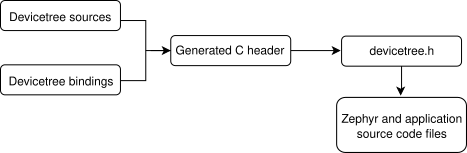
\includegraphics[width=0.8\textwidth]{Include/Figure/software/zephyr_dt_build_flow.png}
	\caption{Simplified \textit{Devicetree} build flow - Source:\cite{dtintro}}
	\label{fig:zephyr_dt_build_flow}
\end{figure}

\warning{\textbf{Warning}: It is necessary to include \textit{devicetree.h} in any  \textit{Zephyr} and application source code that need to access or use the \textit{devicetree}}

\subsubsection{Syntax and structure:}
The human-readable text of the \textit{Devicetree} is called \textit{Device Tree Source} \textit{DTS}.\\
An example \textit{DTS} file is illustrated in the listing \ref{lst:dts_ex}:
\begin{lstlisting}[style=C,label={lst:dts_ex},caption={Example \textit{DTS} File - Source:\cite{dtintro}}]
/{
	a-node {
					subnode_nodelabel: a-sub-node {
							foo = <3>;
					};
	};
};
\end{lstlisting}
\begin{flushleft}
The structure of \textit{devicetree} is composed of three nodes:
\end{flushleft}
\begin{enumerate}
\item A root node: \codeword{/}
\item A node named \codeword{a-node}, which is a child of the root node
\item A node named \codeword{a-sub-node}, which is a child of \codeword{a-node}
\end{enumerate}
\;\\[-40pt]
\subsubsection{Aliases and chosen nodes:}
It possible to refer to a specific node without specifying its entire path using \codeword{aliases} or \codeword{chosen} nodse. An example of \textit{DTS} using both methods is illustrated in listing \ref{lst:aliases_chosen_node}:

\begin{lstlisting}[style=C,label={lst:aliases_chosen_node},caption={Example \textit{DTS} File using \textit{chosen} and \textit{aliases} nodes - Source:\cite{dt_zephyr_user}}]
/ {
	chosen {
				zephyr,console = &uart0;
	};
	aliases {
				my-uart = &uart0;
	};
	soc {
			uart0: serial@12340000 {
                     ...
			};
	};
};
\end{lstlisting}
\;\\[-60pt]
\subsubsection{\textit{zephyr,user} node:}

The \codeword{zephyr,user} node is a very useful node that can be used to describe essentially arbitrary properties that can be retrieve without requiring binding files. It can be compared to a convenient container to store few simple properties.

The \codeword{zephyr,user} node can store three types of properties:
\begin{enumerate}
\item \textbf{Simple values:} numeric or array values that are configurate at build time via \textit{devicetree}
\item \textbf{Devices:} phandles that allows to reconfigure which devices the application uses in simple cases using devicetree overlays
\item \textbf{GPIOs:} Application-specific \textit{GPIOs} that can be reconfigured with a \textit{devicetree} overlay
\end{enumerate}

The three types of properties are illustrated in listings \ref{lst:zephyr_user_simpl_val} to \ref{lst:zephyr_user_gpios}:

\begin{lstlisting}[style=C,label={lst:zephyr_user_simpl_val},caption={Example \textit{zephyr,user} Node - Simple Value Properties - Source:\cite{dt_zephyr_user}}]
/ {
     zephyr,user {
             boolean;
             bytes = [81 82 83];
             number = <23>;
             numbers = <1>, <2>, <3>;
             string = "text";
             strings = "a", "b", "c";
     };
};
\end{lstlisting}

\begin{lstlisting}[style=C,label={lst:zephyr_user_dev},caption={Example \textit{zephyr,user} Node - Devices Properties}]
/ {
     zephyr,user {
             handle = <&gpio0>;
             handles = <&gpio0>, <&gpio1>;
     };
};
\end{lstlisting}

\begin{lstlisting}[style=C,label={lst:zephyr_user_gpios},caption={Example \textit{zephyr,user} Node - \textit{GPIOs} Properties - Source:\cite{dt_zephyr_user}}]
#include <zephyr/dt-bindings/gpio/gpio.h>

/ {
     zephyr,user {
             signal-gpios = <&gpio0 1 GPIO_ACTIVE_HIGH>;
     };
};
\end{lstlisting}

Listings \ref{lst:zephyr_user_retr_sim_val} to \ref{lst:zephyr_user_retr_gpios} illustrates how to retrieve property values from \codeword{zephyr,user} node in application \textit{C/C++} files:

\begin{lstlisting}[style=C,label={lst:zephyr_user_retr_sim_val},caption={Example \textit{zephyr,user} Node - \textit{GPIOs} Properties - Source:\cite{dt_zephyr_user}}]
#define ZEPHYR_USER_NODE DT_PATH(zephyr_user)
DT_PROP(ZEPHYR_USER_NODE, boolean) // 1
DT_PROP(ZEPHYR_USER_NODE, bytes)   // {0x81, 0x82, 0x83}
DT_PROP(ZEPHYR_USER_NODE, number)  // 23
DT_PROP(ZEPHYR_USER_NODE, numbers) // {1, 2, 3}
DT_PROP(ZEPHYR_USER_NODE, string)  // "text"
DT_PROP(ZEPHYR_USER_NODE, strings) // {"a", "b", "c"}
\end{lstlisting}

\begin{lstlisting}[style=C,label={lst:zephyr_user_retr_dev},caption={Example \textit{zephyr,user} Node - \textit{GPIOs} Properties - Source:\cite{dt_zephyr_user}}]
/*
 * Same thing as:
 *
 * ... my_dev = DEVICE_DT_GET(DT_NODELABEL(gpio0));
 */
const struct device *my_device =  DEVICE_DT_GET(DT_PROP(ZEPHYR_USER_NODE, handle));
#define PHANDLE_TO_DEVICE(node_id, prop, idx) \
     DEVICE_DT_GET(DT_PHANDLE_BY_IDX(node_id, prop, idx)),
/*
 * Same thing as:
 *
 * ... *my_devices[] = {
 *         DEVICE_DT_GET(DT_NODELABEL(gpio0)),
 *         DEVICE_DT_GET(DT_NODELABEL(gpio1)),
 * };
 */
const struct device *my_devices[] = {
     DT_FOREACH_PROP_ELEM(ZEPHYR_USER_NODE, handles, PHANDLE_TO_DEVICE)
};
\end{lstlisting}

\begin{lstlisting}[style=C,label={lst:zephyr_user_retr_gpios},caption={Example \textit{zephyr,user} Node - \textit{GPIOs} Properties - Source:\cite{dt_zephyr_user}}]
#include <zephyr/drivers/gpio.h>

#define ZEPHYR_USER_NODE DT_PATH(zephyr_user)

const struct gpio_dt_spec signal =
        GPIO_DT_SPEC_GET(ZEPHYR_USER_NODE, signal_gpios);

/* Configure the pin */
gpio_pin_configure_dt(&signal, GPIO_OUTPUT_INACTIVE);

/* Set the pin to its active level */
gpio_pin_set_dt(&signal, 1);
\end{lstlisting}
\;\\[-50pt]
\subsubsection{Custom Board Creation Process:}

Using the pin assignment of the \textit{LTEWatch} prototype board (table \ref{tab:gpio_ltewatch_board}), a custom devicetree board "\codeword{ltewatch_nrf9160_ns}" was created. The process used to create the custom board is described in \textsc{Nordic Semi.} tutorial video "\textit{Getting started with custom development in nRF Connect SDK}": \url{https://www.youtube.com/watch?v=KSivO9Cf1TE}.\\

The custom board creation process presented in the tutorial is fairly simple:
\begin{enumerate}
\item Duplicate an already existing board with identical SoC. For \textit{LTEWatch}, the \textit{nrf9160dk} development board description, "\codeword{nrf9160dk_nrf9160_ns}", was used.
\item In the duplicate folder, rename each mention of the previous board with the new name of the board. Be careful to rename everything correctly.
\item After renaming, remove any unnecessary definitions or descriptions and adapt the remaining ones to suit the new board hardware.
\end{enumerate}


\subsection{Devicetree overlays:}
In \textit{Zephyr}, \textit{devicetree} overlays are used to reconfigure proprieties defined in \textit{DTS}. The overlay is only used in the application environment and must be described in the root (\textit{src}) directory of the project. To reconfigure a node in the \textit{DT} overlay, à "\&" symbol must be added in front of the node label. Listing \ref{lst:overlay_ex} illustrates an example of \textit{DT} overlay:

\begin{lstlisting}[style=C,label={lst:overlay_ex},caption={\textit{DT} Overlay Example}]
&i2c0 {
       temp: temperature-sensor@76 {
                compatible = "vnd,some-sensor";
                reg = <0x76>;
       };
};
\end{lstlisting}

The propriety described in listing \ref{lst:overlay_ex} can be accessed in the \textit{C/C++} application using the macro: \codeword{DT_ON_BUS(DT_NODELABEL(temp), i2c)}.

\section{\textit{LTEWatch} Application Firmware}
This section describes the \textit{LTEWatch} application firmware that was developed for the prototype board.

\subsection{Application System Configuration:}
The first steps of the firmware development are the application configuration using the project \textit{Kconfig} file and the hardware description using the project's board \textit{Devicetree} overlay file.

\subsubsection{Kconfig:}

The \textit{LTEWatch} application uses multiple drivers and libraries that require to enable \textit{C} and \textit{C++} library from \textit{Zephyr}. The configuration of \textit{C/C++} library is illustrated in the listing \ref{lst:clib_conf}:

\begin{lstlisting}[style=console,label={lst:clib_conf},caption={Application \textit{C} library Configuration}]
# ******************************************** #
# C Library                                    #
# ******************************************** #
CONFIG_NEWLIB_LIBC=y
CONFIG_NEWLIB_LIBC_NANO=n
CONFIG_NEWLIB_LIBC_FLOAT_PRINTF=y

# ******************************************** #
# C++                                          #
# ******************************************** #
CONFIG_CPLUSPLUS=y
CONFIG_LIB_CPLUSPLUS=y
\end{lstlisting}

In order to avoid unexpected comportment during the development state of the firmware, the build optimization is disabled and reset on fatal error is enabled. To use certain drivers, the \textit{C++} library and more particularly \textit{POO}, \textit{Zephyr} requires to enable \textit{C++} exceptions.

\begin{lstlisting}[style=console,label={lst:sys_conf},caption={Application System Configuration}]
# ******************************************** #
# Compiler Optimization                        #
# ******************************************** #
CONFIG_NO_OPTIMIZATIONS=y

# ******************************************** #
# Exception                                    #
# ******************************************** #
CONFIG_EXCEPTIONS=y

# ******************************************** #
# FATAL ERROR Management                       #
# ******************************************** #
CONFIG_RESET_ON_FATAL_ERROR=y
\end{lstlisting}

\textit{Zephyr RTOS} and \textit{XF} requires multiple kind of queues and memory allocation process. For this reason the application memory allocation must be configured. To be more precise, the size of following memory blocks must be configured:
\begin{itemize}
\item Application Main Stack :  Main stack memory allocated for static elements of the application
\item AT Monitor Heap : Heap memory used by the \textit{LTE} Modem to queue dynamic elements
\item Heap Memory Pool : Heap memory used by the executive framework and the \textit{RTOS} for dynamic elements handling, such as events and threads management
\item System Work-queue Stack : Memory allocated to the main system work-queue from \textit{Zephyr}\\
\end{itemize} 

Memory allocation of the \textit{LTEWatch} firmware is described in the listing \ref{lst:memory_conf}:
\begin{lstlisting}[style=console,label={lst:memory_conf},caption={Application Memory Configuration}]
# ********************************************* #
# Heap and stacks                               #
# ********************************************* #
CONFIG_MAIN_STACK_SIZE=12288
CONFIG_AT_MONITOR_HEAP_SIZE=512
CONFIG_HEAP_MEM_POOL_SIZE=8192
#stack size of system k_work queue
CONFIG_SYSTEM_WORKQUEUE_STACK_SIZE=8192
\end{lstlisting}

\subsection{Digital I/O - \textit{GPIO}:}
As mentioned in multiple times, the \textit{LTEWatch} application used several \textit{GPIOs} of the \textit{nRF9160 SiP}. In \textit{Zephyr}, \textit{GPIOs} must be described in the application \textit{Devicetree} and must be enabled in the \textit{Kconfig} file.

\subsubsection{Devicetree:}
To use \textit{GPIOs} in \textit{Zephyr RTOS}, it is simply necessary to enable the \textit{GPIO HAL API} and the \textit{GPIOTE HAL API} in the application \textit{DTS} or \textit{DT} overlay. The \textit{DT} overlay description of \textit{GPIOs} is illustrated in listing \ref{lst:gpio_def}:

\begin{lstlisting}[style=C,label={lst:gpio_def},caption={\textit{DT} \textit{GPIOs} Description}]
&gpiote {
	status = "okay";
};

&gpio0 {
    status = "okay";
};
\end{lstlisting}

\pagebreak

To fully benefit from the \textit{Devicetree} provided by \textit{Zephyr}, some macros are defined using the \codeword{zephyr,user} node. Macros description using \codeword{zephyr,user} node is illustrated in the listing \ref{lst:parma_def}:
\begin{lstlisting}[style=C,label={lst:parma_def},caption={\textit{DT} \textit{GPIOs} Proprieties Description}]
/ {
	zephyr,user {
		// Led
		led-max-number  = <3>;
		// Button
		button-max-number  = <3>;
	 };
};
\end{lstlisting}
\subsubsection{Kconfig:}

Once \textit{GPIOs} are described in the application \textit{Devicetree} it is still necessary to enable \textit{GPIOs} in the application \textit{Kconfig} as shown in listing \ref{lst:gpio_conf}:

\begin{lstlisting}[style=console,label={lst:gpio_conf},caption={Application \textit{GPIOs} Configuration}]
# ********************************************* #
# GPIO                                          #
# ********************************************* #
CONFIG_GPIO=y
\end{lstlisting}

\subsection{Analog Input - \textit{ADC}:}
To use the \textit{ADC}, the process is very similar to that of the \textit{GPIOs}, namely description in the application \textit{Devicetree} and activation of the \textit{API} in the application \textit{Kconfig} .
\subsubsection{Devicetree:}

For the \textit{LTEWatch} application, the \textit{ADC} input \textit{AIN3} with the configuration shown in the listing \ref{lst:adc_def}:

\begin{lstlisting}[style=C,label={lst:adc_def},caption={\textit{DT} \textit{ADC} Description}]
&adc {
	#address-cells = <1>;
	#size-cells = <0>;
    status = "okay";

	channel@0 {
		reg = <0>;
		zephyr,gain = "ADC_GAIN_1_5";
		zephyr,reference = "ADC_REF_INTERNAL";
		zephyr,acquisition-time = <ADC_ACQ_TIME_DEFAULT>;
		zephyr,input-positive = <NRF_SAADC_AIN3>;  // P0.16 = AIN3
		zephyr,resolution = <12>;
	};
};

\end{lstlisting}

As before, some macros are defined in the application \textit{Devicetree} using the \codeword{zephyr,user} node as shown in listing \ref{lst:adc_prop_def}:

\begin{lstlisting}[style=C,label={lst:adc_prop_def},caption={\textit{DT} \textit{ADC} Proprieties Description}]
/ {
	zephyr,user {
		io-channels = <&adc 3>; // P0.16 = AIN3
		// Display
		// Battery Manager
		bat-lvl-gpios	 = <&gpio0 12 GPIO_ACTIVE_HIGH>;
		batlvl-en-gpios   = <&gpio0 11 GPIO_ACTIVE_HIGH>;
		batchrg-int-gpios = <&gpio0 10 GPIO_ACTIVE_LOW>;
	 };
};
\end{lstlisting}
\;\\[-50pt]
\subsubsection{Kconfig:}
On the \textit{nRF9160 SiP} \textit{ADC} requier to enable both \textit{ADC} and \textit{SAADC}, as shown in the listing \ref{lst:adc_conf}:
\begin{lstlisting}[style=console,label={lst:adc_conf},caption={Application \textit{ADC} Configuration}]
# ********************************************* #
# ADC                                           #
# ********************************************* #
CONFIG_ADC=y
CONFIG_ADC_NRFX_SAADC=y
\end{lstlisting}

\subsection{Debug and Logging - \textit{UART}:}
\subsubsection{Devicetree:}
The \textit{UART} description in the application \textit{DT} overlay is described in listing  \ref{lst:uart_def}:

\begin{lstlisting}[style=C,label={lst:uart_def},caption={\textit{DT} \textit{UART} Description}]
&uart0 {
	status = "okay";
	current-speed = <115200>;
	pinctrl-0 = <&uart0_default>;
	pinctrl-1 = <&uart0_sleep>;
	pinctrl-names = "default", "sleep";
};
\end{lstlisting}

The \textit{UART} description from the listing \ref{lst:uart_def} shows new kind of propriety which is the \codeword{pinctrl} node. This node must be defined in a node external to the \textit{UART} node as shown in the listing \ref{lst:uart_pinctrl}:

\begin{lstlisting}[style=C,label={lst:uart_pinctrl},caption={\textit{DT UART} Pinctrl Description}]
&pinctrl {

	uart0_default: uart0_default {
		group1 {
			psels = <NRF_PSEL(UART_TX, 0, 6)>;
		};
		group2 {
			psels = <NRF_PSEL(UART_RX, 0, 7)>;
			bias-pull-up;
		};
	};

	uart0_sleep: uart0_sleep {
		group1 {
			psels = <NRF_PSEL(UART_TX, 0, 6)>,
				<NRF_PSEL(UART_RX, 0, 7)>;
			low-power-enable;
		};
	};
};
\end{lstlisting}

As shown in the listing \ref{lst:uart_pinctrl}, a peripheral can use two different \textit{pinctrl} definitions at the same time. This is a very useful tool that allows you to define different definitions of a specific peripheral depending on the mode it is used in, for example, normal mode and low-power-mode.

\subsubsection{Kconfig:}

When using \textit{UART}, it is possible to enable \textit{UART} interrupt driven configuration using the command described in the listing \ref{lst:uart_conf}:

\begin{lstlisting}[style=console,label={lst:uart_conf},caption={Application \textit{UART} Configuration}]
# ******************************************** #
# UART Interrupt support                       #
# ******************************************** #
CONFIG_UART_INTERRUPT_DRIVEN=y
\end{lstlisting}

Listings \ref{lst:log_conf} and \ref{lst:debug_conf} illustrates the application configuration of \textit{Logging} and \textit{Debugging} options:

\begin{lstlisting}[style=console,label={lst:log_conf},caption={Application \textit{Logging} Configuration}]
# ********************************************** #
# Zephyr/nrf log configuration                   #
# 0 -> off, 1 -> err, 2 ->wrn, 3 -> inf, 4 ->dbg #
# ********************************************** #
CONFIG_CONSOLE=y
CONFIG_LOG=y
CONFIG_LOG_MODE_IMMEDIATE=y
CONFIG_LOG_BACKEND_SHOW_COLOR=y
CONFIG_LOG_INFO_COLOR_GREEN=y
# ******************************************** #
# UART logging                                 #
# ******************************************** #
CONFIG_UART_CONSOLE=y
# ******************************************** #
# RTT logging                                  #
# ******************************************** #
#CONFIG_USE_SEGGER_RTT=y
#CONFIG_RTT_CONSOLE=y
#CONFIG_LOG_BACKEND_RTT=y
\end{lstlisting}

\begin{lstlisting}[style=console,label={lst:debug_conf},caption={Application \textit{Debug} Configuration}]
# ********************************************* #
#  DEBUG settings                               #
# ********************************************* #
CONFIG_DEBUG=y
CONFIG_DEBUG_THREAD_INFO=y
CONFIG_DEBUG_OPTIMIZATIONS=y
CONFIG_DEBUG_INFO=y
CONFIG_DEBUG_COREDUMP=n
\end{lstlisting}

\subsection{Serial Bus - \textit{I2C}:}
\subsubsection{Devicetree:}
The definition and configuration of the \textit{I2C} driver is very similar to that of \textit{UART} and is shown in listings \ref{lst:i2c_def} and \ref{lst:i2c_pinctrl}:
\begin{lstlisting}[style=C,label={lst:i2c_def},caption={\textit{DT I2C} Description}]
&i2c1 {
    compatible = "nordic,nrf-twim";
	status = "okay";
    pinctrl-0 = <&i2c1_default>;
    /* sleep state (only applicable if CONFIG_PM_DEVICE=y) */
    pinctrl-1 = <&i2c1_sleep>;
    /* state assigned to each pinctrl-N property by index */
    pinctrl-names = "default", "sleep";
    clock-frequency = <I2C_BITRATE_STANDARD>;
};

&i2c2 {
    status = "disabled";
};
\end{lstlisting}

\begin{lstlisting}[style=C,label={lst:i2c_pinctrl},caption={\textit{DT I2C} Pinctrl Description}]
&pinctrl {
    /* configuration for i2c1 device, default state */
	i2c1_default: i2c1_default {
		group1 {
			psels = <NRF_PSEL(TWIM_SDA, 0, 8)>,
				<NRF_PSEL(TWIM_SCL, 0, 9)>;
		};
	};

	i2c1_sleep: i2c1_sleep {
		group1 {
			psels = <NRF_PSEL(TWIM_SDA, 0, 8)>,
				<NRF_PSEL(TWIM_SCL, 0, 9)>;
			low-power-enable;
		};
	};
};
\end{lstlisting}

\subsubsection{Kconfig:}
Similar to the \textit{ADC} configuration, the \textit{I2C} configuration on the \textit{nRF9160} requires to enable both \textit{I2C} and \textit{I2C NRFX} \textit{APIs}, as shown in the listing \ref{lst:i2c_conf}:
\begin{lstlisting}[style=console,label={lst:i2c_conf},caption={Application \textit{I2C} Configuration}]
# ********************************************* #
# I2C                                           #
# ********************************************* #
CONFIG_I2C=y
CONFIG_I2C_NRFX=y
\end{lstlisting}

\subsection{Serial Bus - \textit{SPI}:}
Nearly identical to the definition and configuration of the \textit{I2C} \textit{API}, the \textit{SPI} definition and configuration is illustrated in listings \ref{lst:spi_def} to \ref{lst:spi_conf}:
\subsubsection{Devicetree:}
The \textit{DT} application overlay has a small difference from the \textit{I2C} which is the additional \textit{LS0XX} display driver definition as shown in the listing \ref{lst:spi_def}. The \textit{LS0XX} display driver definition is used to configure the display specifications such as width, height and serial communication max frequency.

\begin{lstlisting}[style=C,label={lst:spi_def},caption={\textit{DT SPI} Description}]
&spi3 {
    status = "disabled";
};

&spi2 {
	compatible = "nordic,nrf-spim";
	status = "okay";
    cs-gpios = <&gpio0 28 GPIO_ACTIVE_HIGH>, 	//Display scs
				<&gpio0 20 GPIO_ACTIVE_LOW>;	//Accelerometer scs
	pinctrl-0 = <&spi2_default>;
	pinctrl-1 = <&spi2_sleep>;
	pinctrl-names = "default", "sleep";
	ls0xx: ls0xx@0 {
		compatible = "sharp,ls0xx";
		label = "DISPLAY";
		spi-max-frequency = <2000000>;
		width = <160>;
		height = <68>;
		reg = <0>;
	};
};
\end{lstlisting}

\pagebreak

\begin{lstlisting}[style=C,label={lst:spi_pinctrl},caption={\textit{DT SPI} Pinctrl Description}]
&pinctrl {
	spi2_default: spi2_default {
		group1 {
			psels = <NRF_PSEL(SPIM_SCK, 0, 30)>,
					<NRF_PSEL(SPIM_MISO, 0, 29)>,
					<NRF_PSEL(SPIM_MOSI, 0, 31)>;
		};
	};

	spi2_sleep: spi2_sleep {
		group1 {
			psels = <NRF_PSEL(SPIM_SCK, 0, 30)>,
					<NRF_PSEL(SPIM_MISO, 0, 29)>,
					<NRF_PSEL(SPIM_MOSI, 0, 31)>;
			low-power-enable;
		};
	};
};
\end{lstlisting}
\;\\[-60pt]
\subsubsection{Kconfig:}

\begin{lstlisting}[style=console,label={lst:spi_conf},caption={Application \textit{SPI} Configuration}]
# SPI                                           #
# ********************************************* #
CONFIG_SPI=y
\end{lstlisting}
\;\\[-50pt]
\subsection{Motor Driver:}
The motor driving functionality of the \textit{LTEWatch} application requires macros definitions to describe \textit{GPIOs} pin used to drive motors and also uses \textit{aliases} node to share \textit{GPIOs} that are also defined as LEDs. The definition of the \codeword{zephyr,user} node and the \codeword{aliases} node is illustrated in the listing \ref{lst:motor_prop_def}:
\subsubsection{Devicetree:}

\begin{lstlisting}[style=C,label={lst:motor_prop_def},caption={\textit{DT Motor} Proprieties and Aliases Description}]
/ {
	zephyr,user {
		// Clock Motors
		motor-max-number  = <3>;
		motor-d1m1-gpios  = <&gpio0 0 GPIO_ACTIVE_HIGH>;
		motor-d1com-gpios = <&gpio0 1 GPIO_ACTIVE_HIGH>;
		motor-d1m2-gpios  = <&gpio0 2 GPIO_ACTIVE_HIGH>;
		motor-d2m1-gpios  = <&gpio0 5 GPIO_ACTIVE_HIGH>;
		motor-d2com-gpios = <&gpio0 4 GPIO_ACTIVE_HIGH>;
		motor-d2m2-gpios  = <&gpio0 3 GPIO_ACTIVE_HIGH>;
	 };
	 aliases {
		motord3m1  = &led0;
		motord3com = &led1;
		motord3m2  = &led2;
	};
};
\end{lstlisting}
\subsubsection{Kconfig:}
The stepper motors used to display the time are driven using time-critical control signals. To ensure the accuracy and consistency of the motor control signal, the signal timing uses the \textit{RTC} as time reference. The \textit{RTC} driver configuration for the \textit{nRF9160} is shown in the \ref{lst:rtc_conf} listing:
\begin{lstlisting}[style=console,label={lst:rtc_conf},caption={Application \textit{RTC} Configuration}]
# ******************************************** #
# RTC Config	                                #
# ******************************************** #
CONFIG_NRFX_RTC0=y
# To run in non-secure mode, you need to add RTC0 to spm.c
CONFIG_COMPILER_OPT="-DNRFX_RTC_ENABLED=1 -DNRFX_RTC0_ENABLED=1"

\end{lstlisting}

\subsection{\textit{Display}:}

\subsubsection{Devicetree:}

\begin{lstlisting}[style=C,label={lst:lcd_def},caption={\textit{DT} \textit{Display} Description}]
/ {
	chosen {
		zephyr,display = &ls0xx;
	};

};
\end{lstlisting}

\begin{lstlisting}[style=C,label={lst:disp_prop_def},caption={\textit{DT Display} Proprieties Description}]
/ {
	zephyr,user {
		// Display
		disp-en-gpios = <&gpio0 27 GPIO_ACTIVE_HIGH>;
	 };
};
\end{lstlisting}
\;\\[-60pt]
\subsubsection{Kconfig:}

\begin{lstlisting}[style=console,label={lst:disp_conf},caption={Application \textit{Display} Configuration}]
# ******************************************** #
# Config Display                               #
# ******************************************** #
CONFIG_LV_Z_MEM_POOL_NUMBER_BLOCKS=16
CONFIG_DISPLAY=y
CONFIG_LVGL=y
CONFIG_LV_MEM_CUSTOM=y
CONFIG_LV_USE_LABEL=y
CONFIG_LV_USE_IMG=y
CONFIG_LV_FONT_DEFAULT_MONTSERRAT_16=y
CONFIG_LV_COLOR_DEPTH_1=y
CONFIG_LS0XX=y
CONFIG_LV_TXT_ENC_UTF8=y
\end{lstlisting}

\subsection{\textit{GNSS} Receiver:}

\subsubsection{Devicetree:}

\begin{lstlisting}[style=C,label={lst:gnss_def},caption={\textit{DT GNSS} Proprieties Description}]
/ {
	zephyr,user {
		// GNSS Receiver
		gps-rst-gpios = <&gpio0 25 GPIO_ACTIVE_LOW>;
		gps-en-gpios  = <&gpio0 26 GPIO_ACTIVE_HIGH>;
	 };
};
\end{lstlisting}
\;\\[-60pt]
\subsubsection{Kconfig:}

\begin{lstlisting}[style=console,label={lst:gnss_conf},caption={Application \textit{GNSS} Configuration}]
# ********************************************* #
# UBXLIX configuration (GNSS)                   #
# ********************************************* #
CONFIG_UBXLIB=y
CONFIG_UBXLIB_GNSS=y
CONFIG_UBXLIB_CELL=y
CONFIG_UBXLIB_TEST=n
\end{lstlisting}

\subsection{\textit{LTE} Modem \& \textit{MQTT}:}

\subsubsection{Kconfig:}

\begin{lstlisting}[style=console,label={lst:mqtt_def},caption={Application \textit{LTE/MQTT} Configuration}]
# ********************************************* #
# Networking                                    #
# ********************************************* #
CONFIG_NETWORKING=y
CONFIG_NET_NATIVE=n
CONFIG_NET_SOCKETS_OFFLOAD=y
CONFIG_NET_SOCKETS=y
CONFIG_NET_SOCKETS_POSIX_NAMES=y

# ********************************************* #
# LTE configuration                             #
# ********************************************* #
CONFIG_LTE_LINK_CONTROL=y
CONFIG_LTE_AUTO_INIT_AND_CONNECT=n

# Modem library
CONFIG_NRF_MODEM_LIB=y

# Antenna
CONFIG_MODEM_ANTENNA=y
CONFIG_MODEM_ANTENNA_AT_MAGPIO="AT%XMAGPIO=1,0,0,1,1,1574,1577"
CONFIG_MODEM_ANTENNA_AT_COEX0="AT%XCOEX0=1,1,1565,1586"

# ********************************************* #
# MQTT configuration                            #
# ********************************************* #
# MQTT Zephyr configuration
CONFIG_MQTT_LIB=y
CONFIG_MQTT_CLEAN_SESSION=y
CONFIG_NRF_CLOUD_MQTT=n
# MQTT custom configuration
CONFIG_MQTT_KEEPALIVE=20
# MAX sockets simultaneously open
CONFIG_POSIX_MAX_FDS=9
\end{lstlisting}

\section{Overview of \textit{LTEWatch} Application Software}

To provide a better idea of the developed small watch application, the project structure is illustrated in project trees \ref{tree:LTEWatchAppStruct} to \ref{tree:LTEWatchAppStruct6}.\\

In the next project trees, the flowing color-code is used:
\begin{enumerate}
\item \textbf{\textcolor{blue}{Blue}} : Unmodified source files imported from other applications
\item \textbf{\textcolor{orange}{Orange}} : Slightly modified source files imported from other applications, most current modification is adaptation to \textit{Zephyr RTOS}
\item \textbf{\textcolor{red}{Red}} :  New files created for the \textit{LTEWatch} application
\end{enumerate}

\tree{0.5}{LTEWatchAppStruct}{\textit{LTEWatch} Application Project Structure}{%
.1 src/.
.2 app/.
.3 config/.
.3 \textcolor{red}{appfactory.cpp}. %\DTcomment{\rmfamily\color{orange}{\# .git}}.
.3 \textcolor{blue}{eventid.h}.
.3 \textcolor{red}{picowatch.h}.
.3 \textcolor{red}{picowatch.cpp}.
.2 board/.
.2 core/.
.3 \textcolor{orange}{factory.h}.
.3 \textcolor{orange}{factory.cpp}.
.3 \textcolor{orange}{main.cpp}.
.2 library/.
.3 \textcolor{red}{mcu/}.
.3 \textcolor{red}{mdw/}.
.3 project-config.
.4 \textcolor{orange}{debug-config.h}.
.4 \textcolor{orange}{platform-config.h}.
.3 \textcolor{blue}{xf/}.
}

\tree{0.5}{LTEWatchAppStruct2}{\textit{LTEWatch} Application Project Structure - \textit{mcu}}{%
.1 src/library/mcu/.
.2 hal/.
.3 battery/.
.4 \textcolor{red}{bathal.h}.
.4 \textcolor{red}{bathal.cpp}.
.3 \textcolor{blue}{critical/}.
.3 gpio/.
.4 \textcolor{orange}{gpiohal.h}.
.4 \textcolor{orange}{gpiohal.cpp}.
.4 \textcolor{orange}{ledhal.h}.
.4 \textcolor{orange}{ledhal.cpp}.
.3 motor/.
.4 \textcolor{orange}{motordriverhal.h}.
.4 \textcolor{orange}{motordriverhal.cpp}.
.2 tools/.
.3 \textcolor{orange}{sdktool.h}.
.3 \textcolor{orange}{dktool.cpp}.
}

\tree{0.5}{LTEWatchAppStruct3}{\textit{LTEWatch} Application Project Structure - \textit{mdw}}{%
.1 src/library/mdw/.
.2 common/.
.2 partners/.
.3 battery/.
.4 config/.
.5 \textcolor{red}{batt-config.h}.
.4 driver/.
.5 \textcolor{red}{drv\_bq25180.h}.
.4 \textcolor{red}{batterymanager.h}.
.4 \textcolor{red}{batterymanager.cpp}.
.4 \textcolor{red}{ibatteryobserver.h}.
.3 calendar/.
.4 config/.
.5 \textcolor{blue}{calendar-config.h}.
.4 interface/.
.5 \textcolor{blue}{calendarobserver.h}.
.4 XF/.
.5 \textcolor{blue}{calendarevent.h}.
.4 \textcolor{red}{calendar.h}.
.4 \textcolor{red}{calendar.cpp}.
.4 \textcolor{blue}{datetime.h}.
.4 \textcolor{blue}{datetime.cpp}.
.3 motor/.
}

\tree{0.5}{LTEWatchAppStruct4}{\textit{LTEWatch} Application Project Structure - \textit{mdw/partners/motor}}{%
.1 src/library/mdw/partners/motor/.
.2 config/.
.3 motor-config.h.
.2 interface/.
.3 \textcolor{blue}{motorctrlobserver.h}.
.3 \textcolor{blue}{motordriverobserver.h}.
.2 XF/.
.3 \textcolor{blue}{motorendevent.h}.
.3 \textcolor{blue}{motorevent.h}.
.3 \textcolor{blue}{motorinitevent.h}.
.2 \textcolor{blue}{motor.h}.
.2 \textcolor{blue}{motor.cpp}.
.2 \textcolor{blue}{motorcontroller.h}.
.2 \textcolor{blue}{motorcontroller.cpp}.
.2 \textcolor{blue}{motordriver.h}.
.2 \textcolor{blue}{motordriver.cpp}.
.2 \textcolor{blue}{motorid.h}.
}

\tree{0.5}{LTEWatchAppStruct5}{\textit{LTEWatch} Application Project Structure - \textit{mdw/common}}{%
.1 src/library/mdw/common/.
.2 button/.
.3 config/.
.4 \textcolor{blue}{button-config.h}.
.3 interface/.
.4 \textcolor{blue}{buttonobserver.h}.
.4 \textcolor{blue}{button.h}.
.4 \textcolor{orange}{buttoncontroller.h}.
.4 \textcolor{orange}{buttoncontroller.cpp}.
.4 \textcolor{blue}{buttonid.h}.
.2 \textcolor{blue}{core/}.
.2 \textcolor{blue}{critical/}.
.2 display/.
.3 config/.
.4 \textcolor{red}{disp-config.h}.
.3 \textcolor{red}{dispcontroller.h}.
.3 \textcolor{red}{dispcontroller.cpp}.
.2 gnss/.
.3 config/.
.4 \textcolor{red}{gnss-config.h}.
.3 \textcolor{red}{gnsscontroller.h}.
.3 \textcolor{red}{gnsscontroller.cpp}.
.3 \textcolor{red}{ignssobserver.h}.
}

\tree{0.5}{LTEWatchAppStruct6}{\textit{LTEWatch} Application Project Structure - \textit{mdw/common}}{%
.1 src/library/mdw/common/.
.2 gpio/.
.3 \textcolor{blue}{config/}.
.3 \textcolor{blue}{interface/}.
.3 \textcolor{blue}{XF/}.
.3 \textcolor{blue}{basecontroller.h}.
.3 \textcolor{blue}{basecontroller.cpp}.
.3 \textcolor{blue}{gpio.h}.
.3 \textcolor{blue}{gpio.cpp}.
.3 \textcolor{orange}{gpiocontroller.h}.
.3 \textcolor{orange}{gpiocontroller.cpp}.
.3 \textcolor{blue}{gpioid.h}.
.3 \textcolor{orange}{ledcontroller.h}.
.3 \textcolor{orange}{ledcontroller.cpp}.
.2 \textcolor{blue}{lte/}.
.2 \textcolor{blue}{mqtt/}.
.2 picoxf/.
.3 \textcolor{orange}{picoevent.h}.
.3 \textcolor{orange}{picoevent.cpp}.
.3 \textcolor{orange}{picoireactive.h}.
.3 \textcolor{orange}{picoxf.h}.
.3 \textcolor{orange}{picoxf.cpp}.
.2 \textcolor{blue}{pool/}.
}

As shown in project trees \ref{tree:LTEWatchAppStruct} to \ref{tree:LTEWatchAppStruct6} many files are unmodified or slightly modified. Those files were provide by \textsc{Patrice Rudaz} from the \textit{HEVS} in order to make the software application development faster and easier. Those files come from two different projects from \textsc{Patrice Rudaz}: 
\begin{itemize}
\item MoskitoWatch Application
\item BikeBox Application\\
\end{itemize}

The unmodified files will not be presented in this chapter. The slightly modified files are most often just adapted for \textit{Zephyr RTOS} by replacing any timers with the \textit{Zephyr} kernel timer \textit{API} \textit{k\_timer} or replacing old \textit{GPIO} \textit{API} used by the new \textit{GPIO} and \textit{GPIOTE} \textit{APIs} from \textit{Zephyr RTOS} and also the implementation of the \textit{RTC} \textit{API} of \textit{MotorDriverHal} for \textit{Zephyr RTOS}. 

\pagebreak

\section{Battery Manager}
The \textit{Batter Manager} module implement features required to use the \textit{BQ25180} battery  charger. For this module a compatible driver for the \textit{BQ25180} \textit{drv\_bq25180.h} and two classes \textit{BatHal} and \textit{BatteyManager} were created.

\subsection{BatteryManager Class Diagram:}

Figure \ref{fig:batterymanager} illustrates the class diagram of \textit{BatteryManager}: 

\begin{figure}[H]
	\centering
	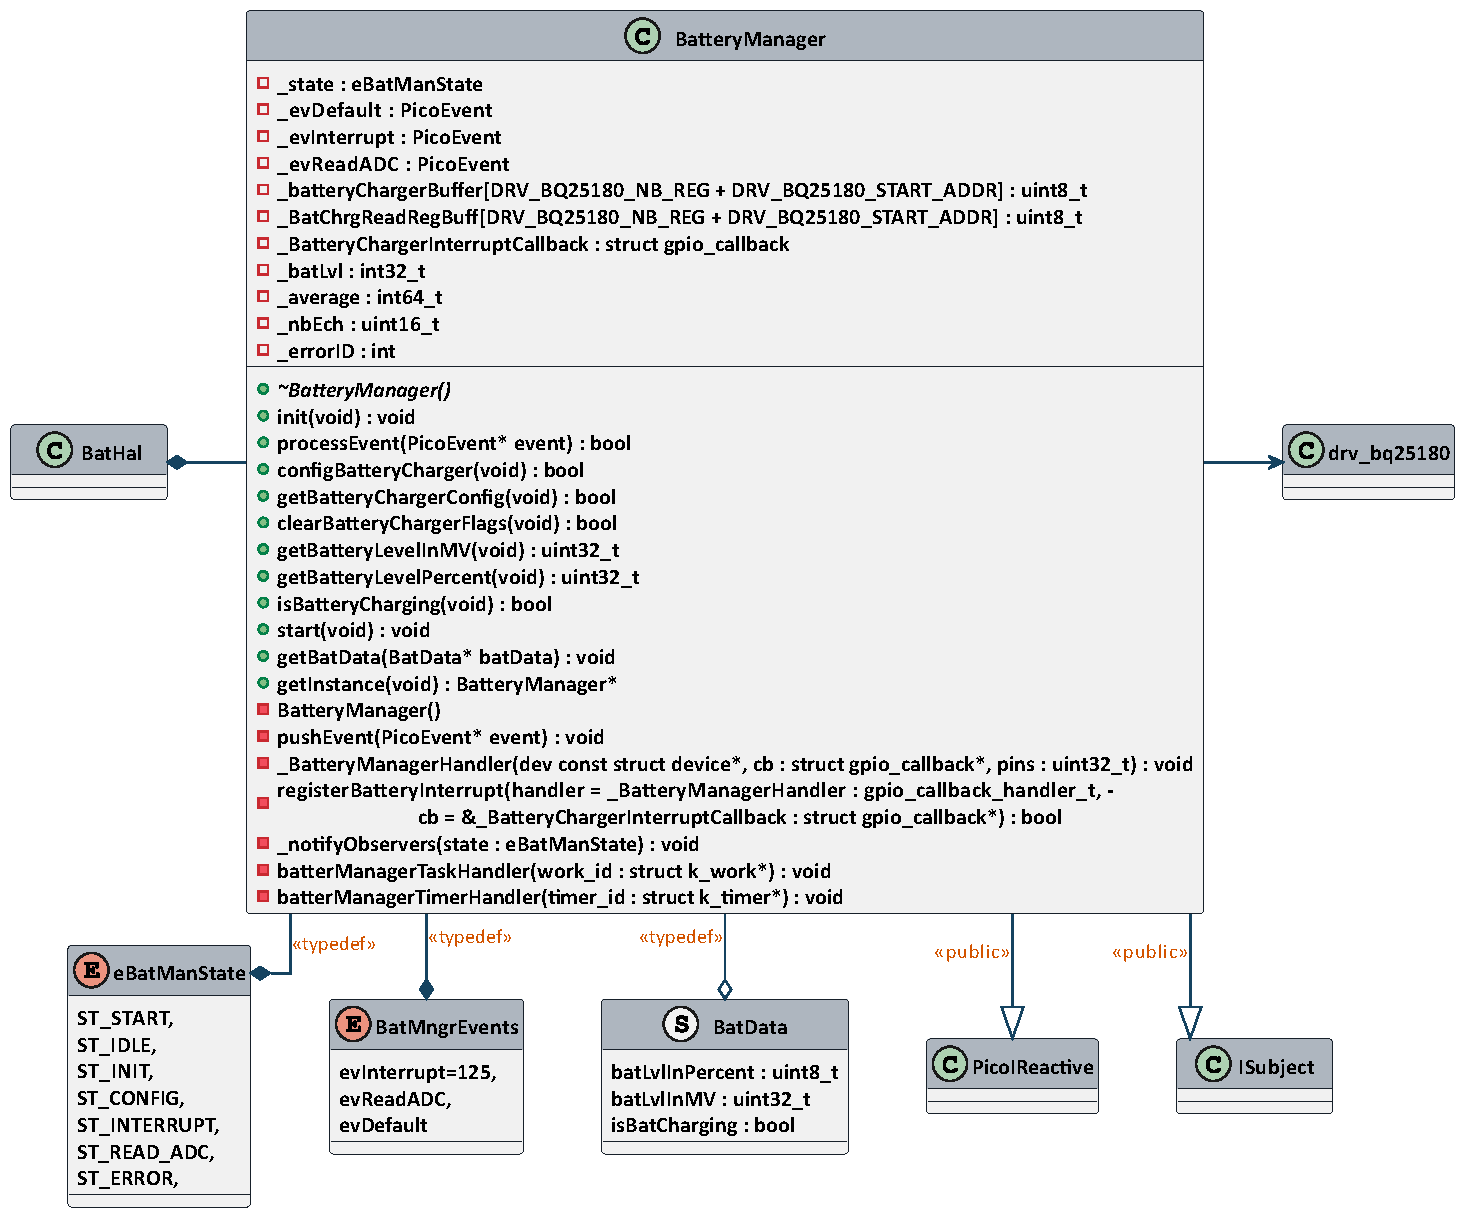
\includegraphics[width=1\textwidth]{Include/Figure/software/class/batterymanager.pdf}
	\caption{\textit{BatteryManager} Class Diagram}
	\label{fig:batterymanager}
\end{figure}

\subsection{Battery Charger Driver - \textit{drv\_bq25180.h}}
The \textit{drv\_bq25180.h} file is a driver for the \textit{BQ25180}. This driver provides many useful elements to implement the \textit{BQ25180} more easily.

\pagebreak
\subsection{Battery Hardware Abstraction Layer (BatHal)}

Figure \ref{fig:bathal} illustrates the class diagram of \textit{BatHal}: 

\begin{figure}[H]
	\centering
	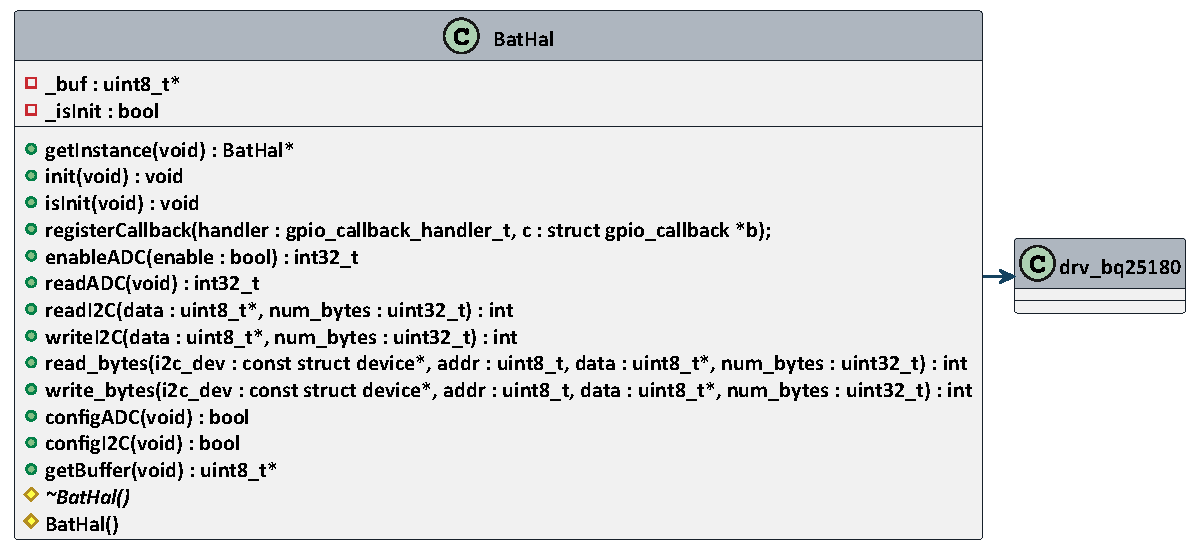
\includegraphics[width=0.9\textwidth]{Include/Figure/software/class/bathal.pdf}
\caption{\textit{BatHal} Class Diagram}
	\label{fig:bathal}
\end{figure}

Functions described in figure \ref{fig:bathal} are required by the \textit{BatteryManager} class to  to interface with the \textit{BQ25180} battery charger and the \textit{ADC} input connected to the battery level monitoring circuit.

\subsection{BatteryManager State Diagram:}

Figure \ref{fig:batteryManagerstate} illustrate the state diagram of \textit{BtteryManger} class:

\begin{figure}[H]
	\centering
	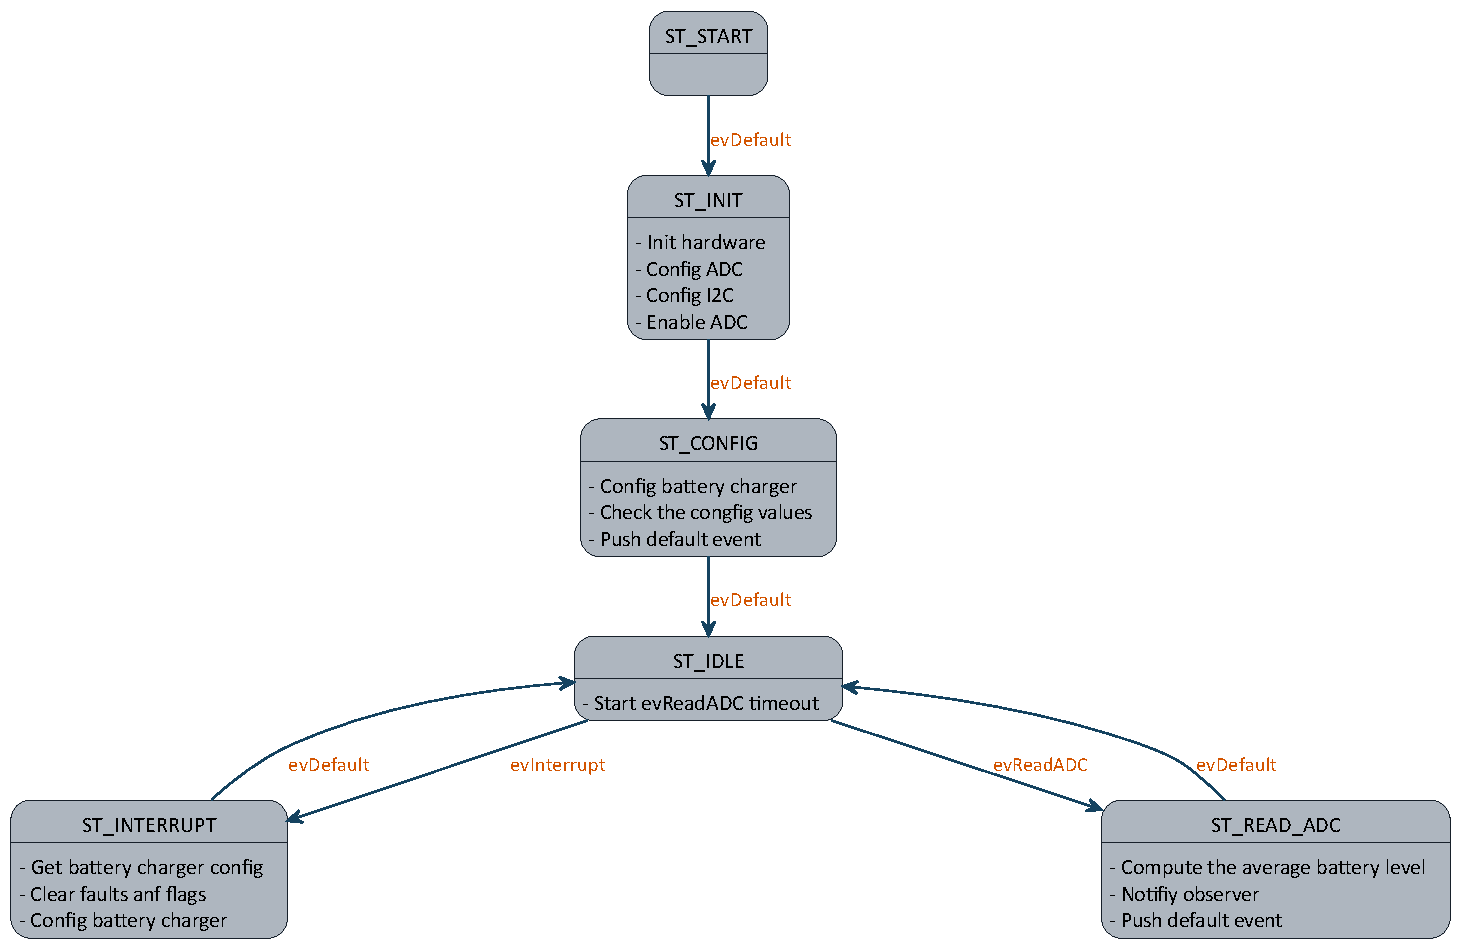
\includegraphics[width=0.9\textwidth]{Include/Figure/software/state/batteryManager.pdf}
	\caption{\textit{BatteryManager} State Diagram}
	\label{fig:batteryManagerstate}
\end{figure}

\section{Display}

\subsection{\textit{DispController} Class Diagram}

Figure \ref{fig:dispcontroller} illustrates the class diagram of \textit{DispController}: 

\begin{figure}[H]
	\centering
	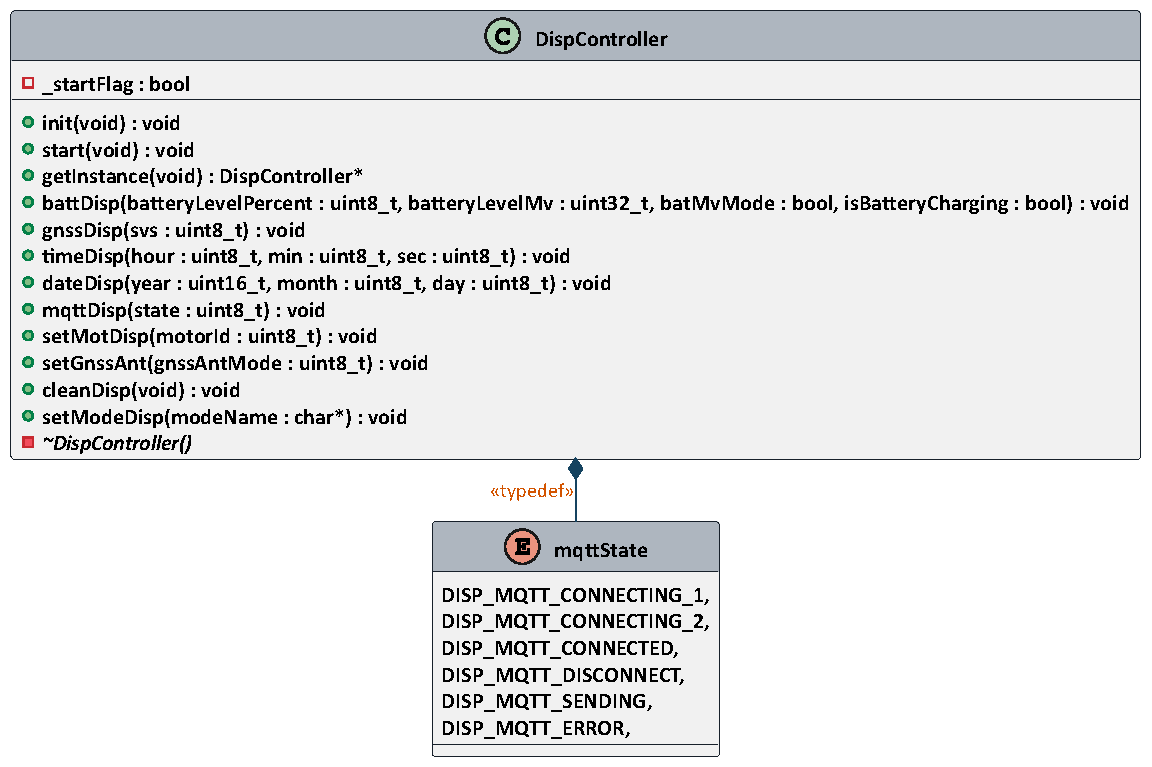
\includegraphics[width=1\textwidth]{Include/Figure/software/class/dispcontroller.pdf}
	\caption{\textit{DispController} Class Diagram}
	\label{fig:dispcontroller}
\end{figure}

\pagebreak
\section{\textit{GNSS} Receiver}
\subsection{\textit{GNSS} controller}
\textit{GnssController} application is based on the \textit{msg\_main.c} from the \textit{ubxlib} repository: \url{https://github.com/u-blox/ubxlib/blob/master/example/gnss/msg_main.c}
\subsubsection{\textit{GnssController} Class Diagram}

Figure \ref{fig:gnsscontroller} illustrates the class diagram of \textit{GnssController}: 

\begin{figure}[H]
	\centering
	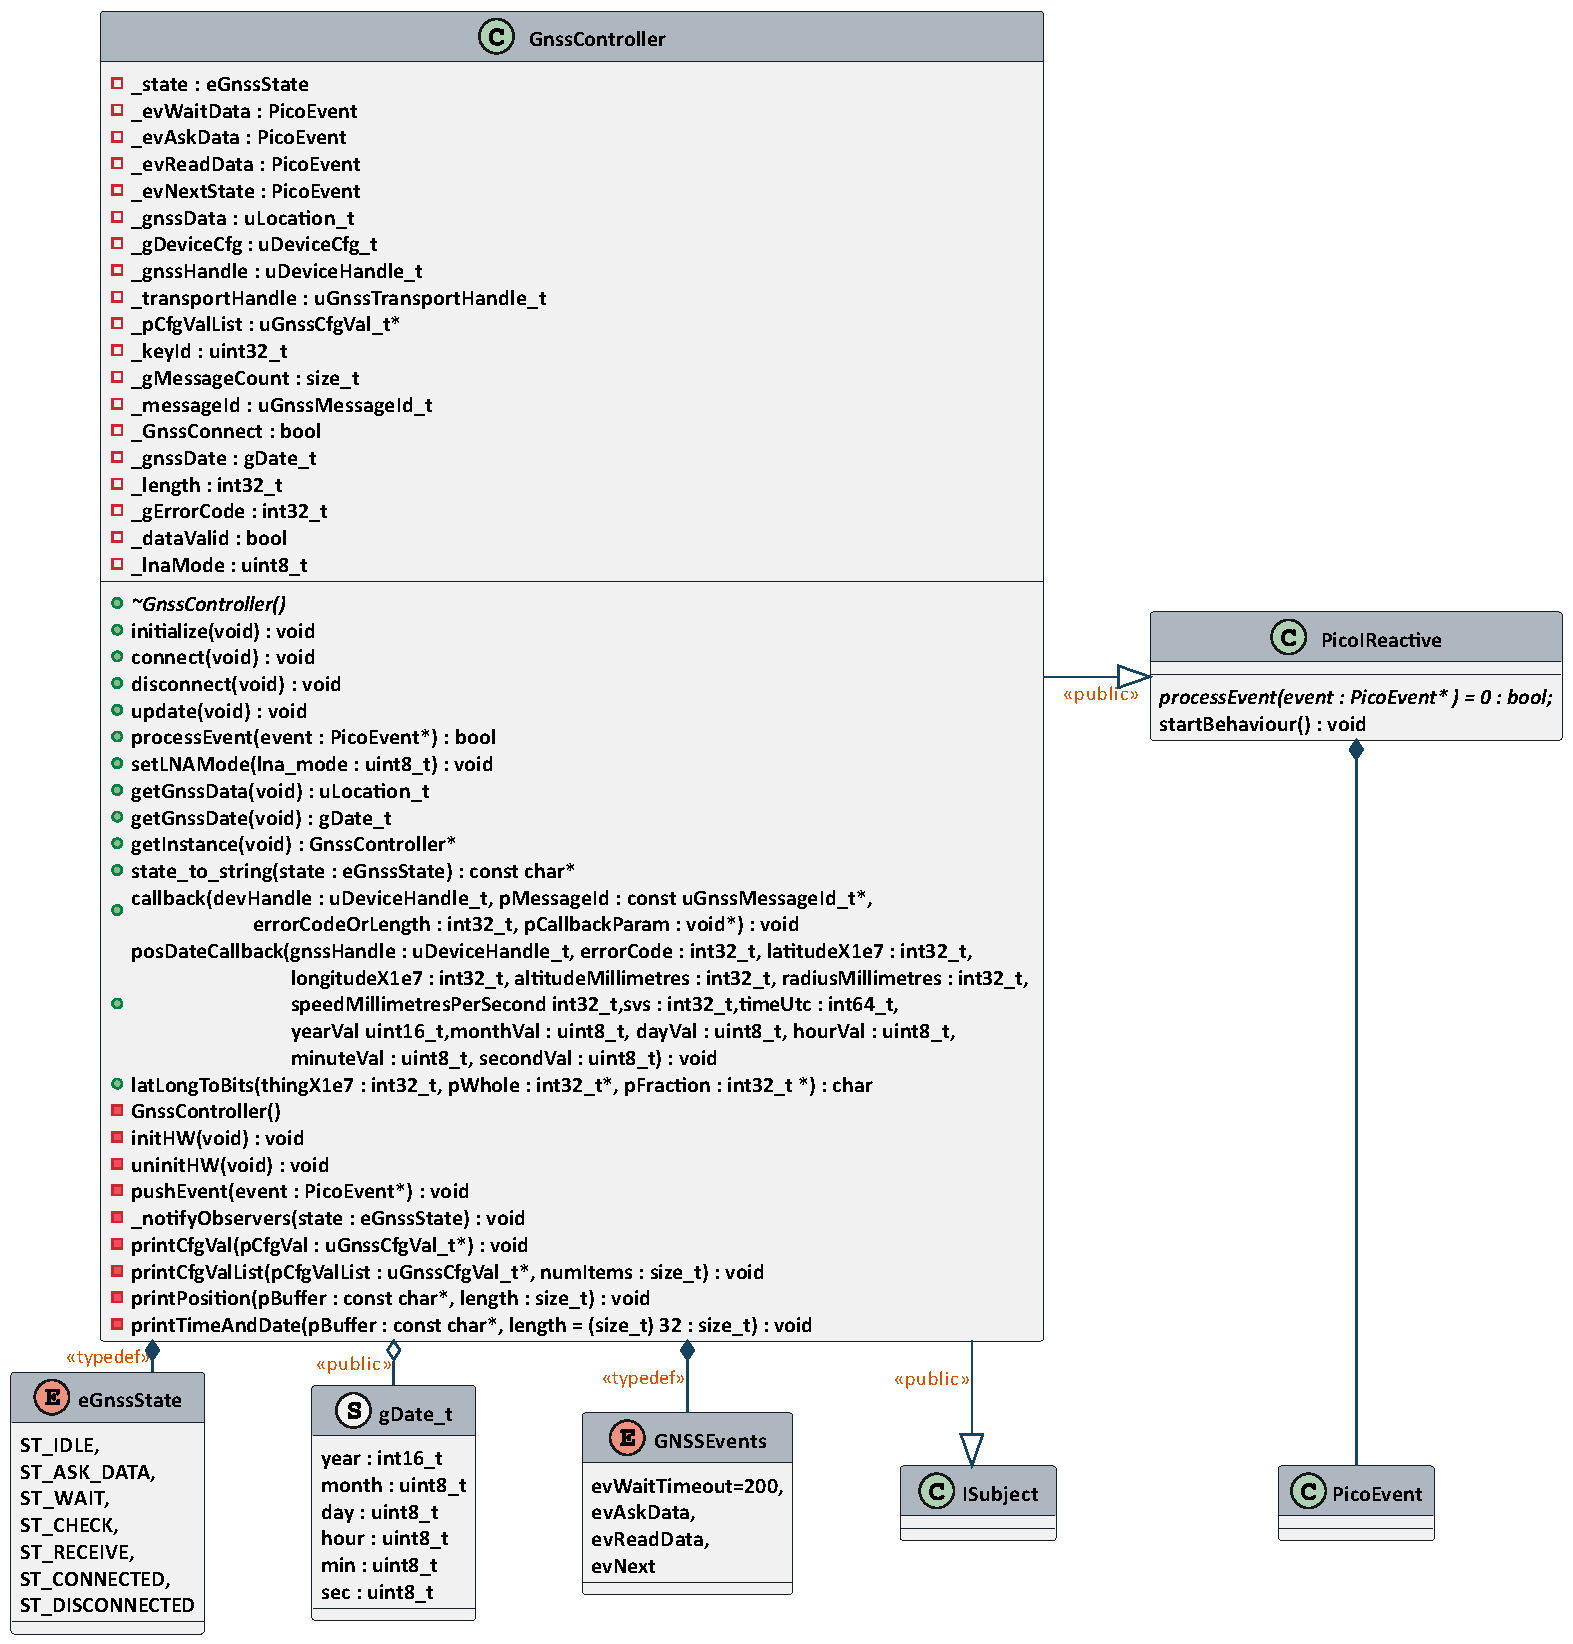
\includegraphics[width=1\textwidth]{Include/Figure/software/class/gnsscontroller.pdf}
	\caption{\textit{GnssController} Class Diagram}
	\label{fig:gnsscontroller}
\end{figure}

\pagebreak
\subsubsection{\textit{GnssController} State Diagram}

Figure \ref{fig:gnssController} illustrates the state diagram of \textit{GnssController} class: 

\begin{figure}[H]
	\centering
	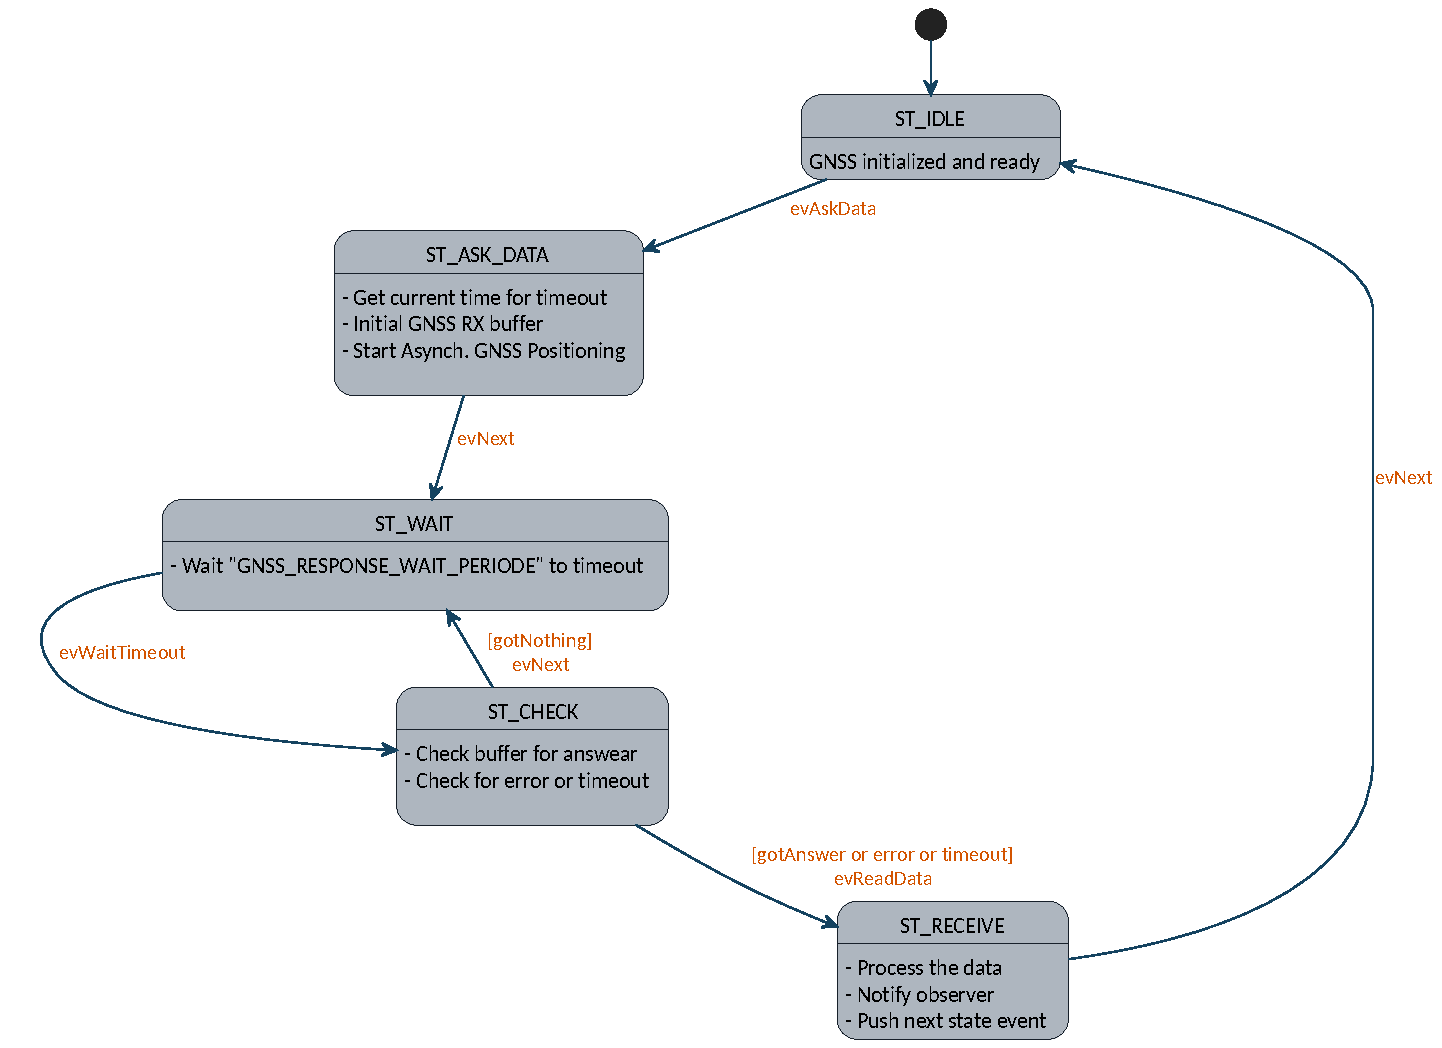
\includegraphics[width=1\textwidth]{Include/Figure/software/state/gnssController.pdf}
	\caption{\textit{GnssController} State Diagram}
	\label{fig:gnssController}
\end{figure}

\pagebreak

\section{\textit{LTEWatch} Application}
\subsection{\textit{Factory} Class Diagram}

Figure \ref{fig:factory} illustrates the class diagram of \textit{Factory}: 

\begin{figure}[H]
	\centering
	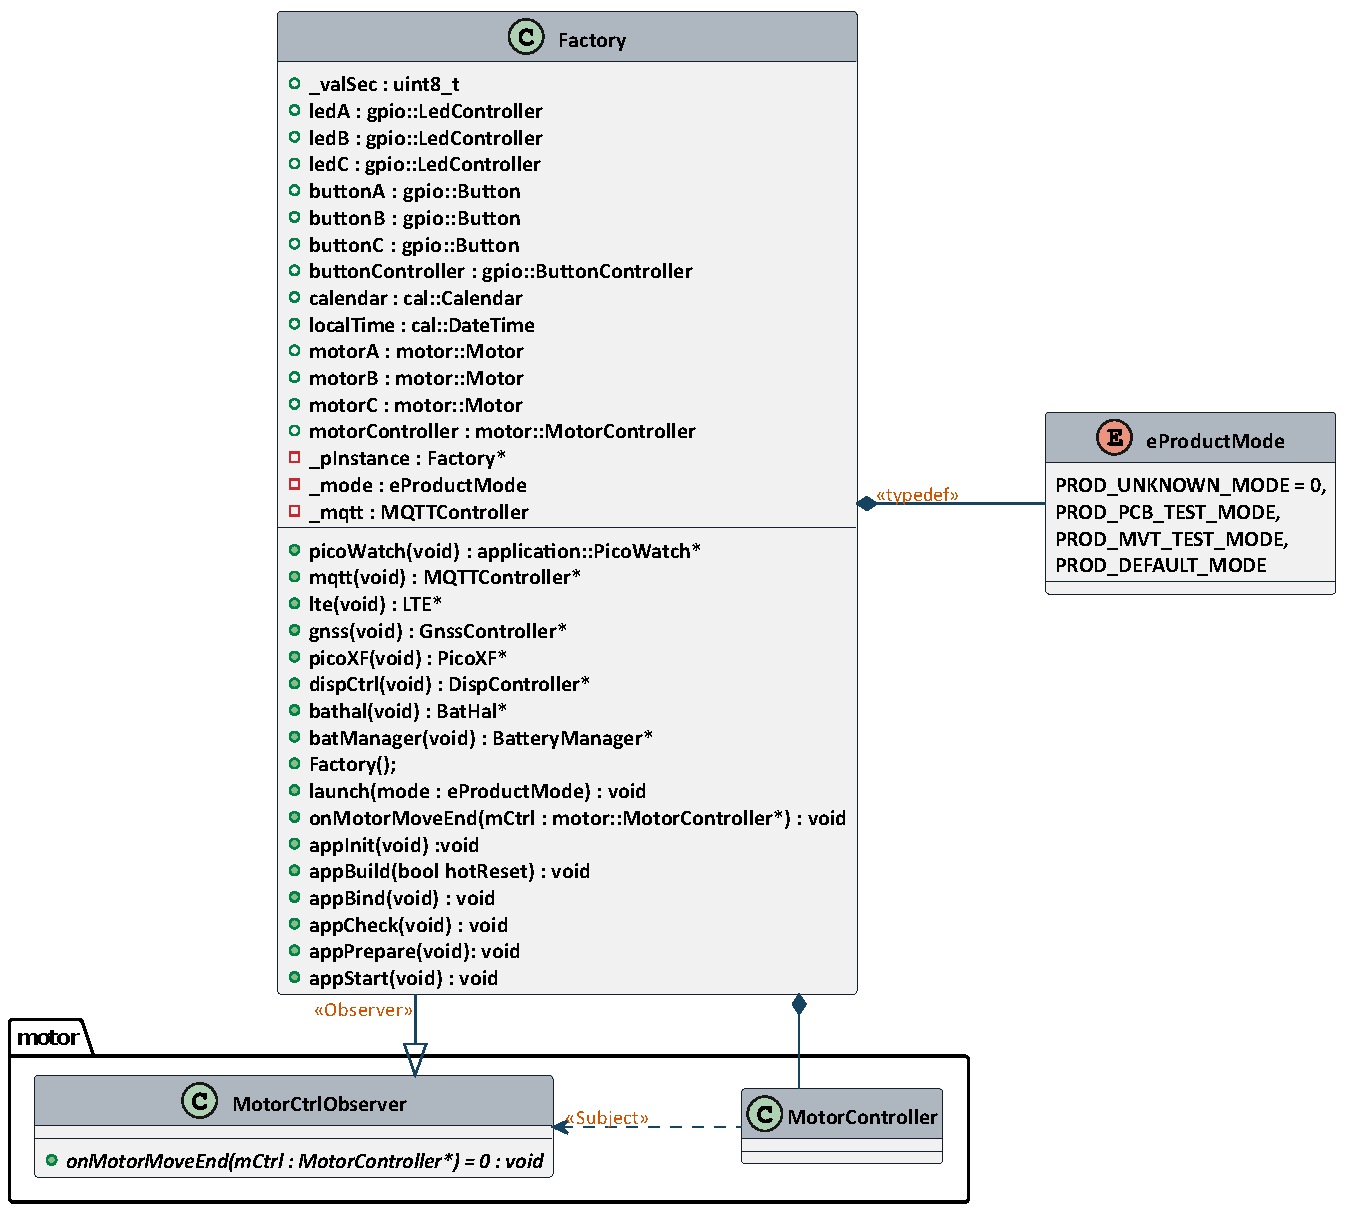
\includegraphics[width=1\textwidth]{Include/Figure/software/class/factory.pdf}
	\caption{\textit{Factory} Class Diagram}
	\label{fig:factory}
\end{figure}


\pagebreak

\subsection{\textit{PicoWatch} Class Diagram}
\textit{PicoWatch} is the main class of the \textit{LTEWatch} firmware. This class controls all modules of the application.\\

Figure \ref{fig:picowatch_small_1} and figure \ref{fig:picowatch_small_2} illustrate the class diagrams of \textit{PicoWatch}: 

\begin{figure}[H]
	\centering
	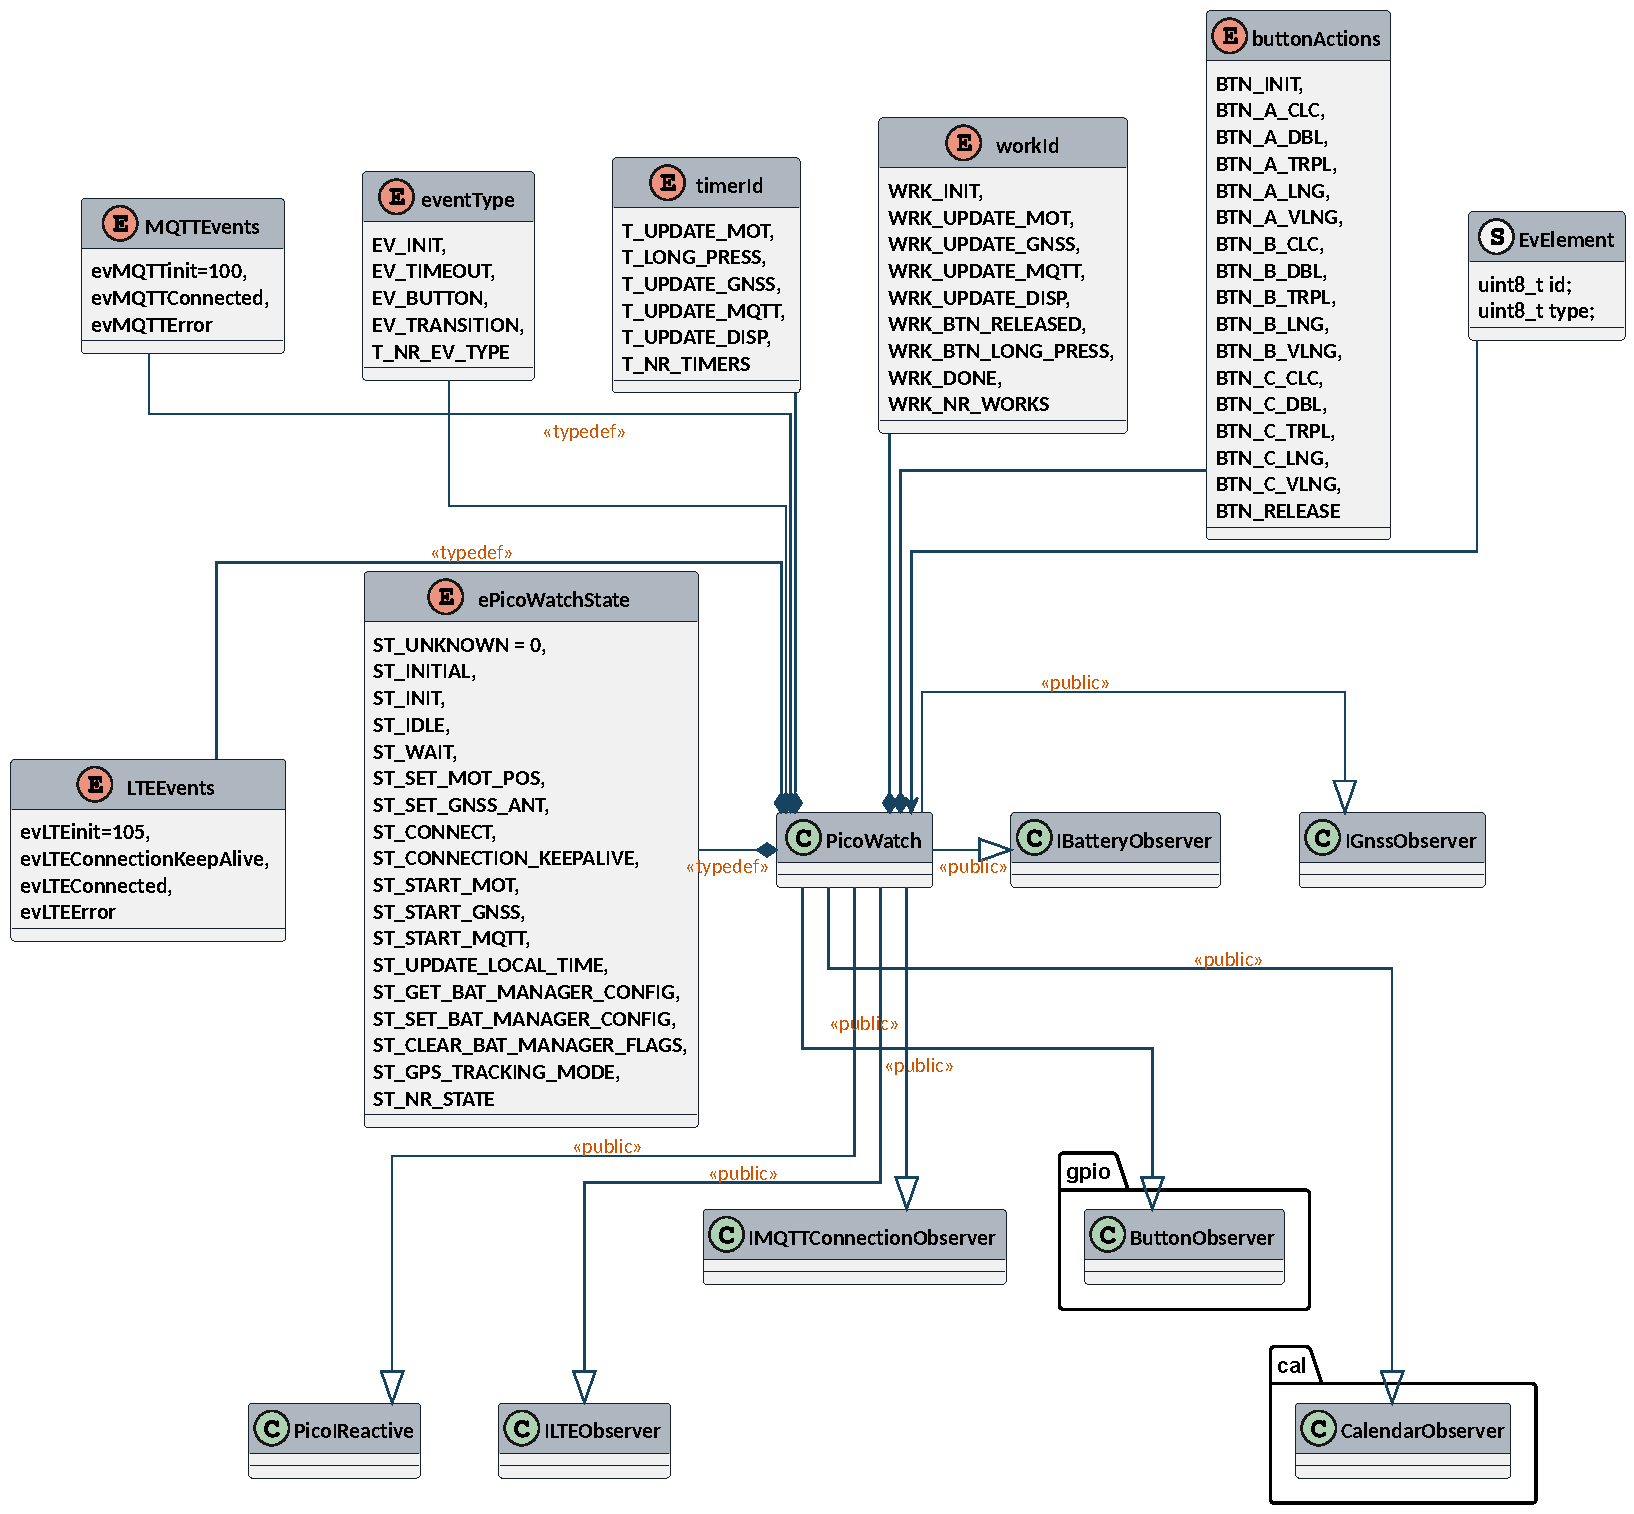
\includegraphics[width=1\textwidth]{Include/Figure/software/class/picowatch_small_2.pdf}
	\caption{\textit{PicoWatch} Class Diagram - Part 1}
	\label{fig:picowatch_small_1}
\end{figure}

\begin{figure}[H]
	\centering
	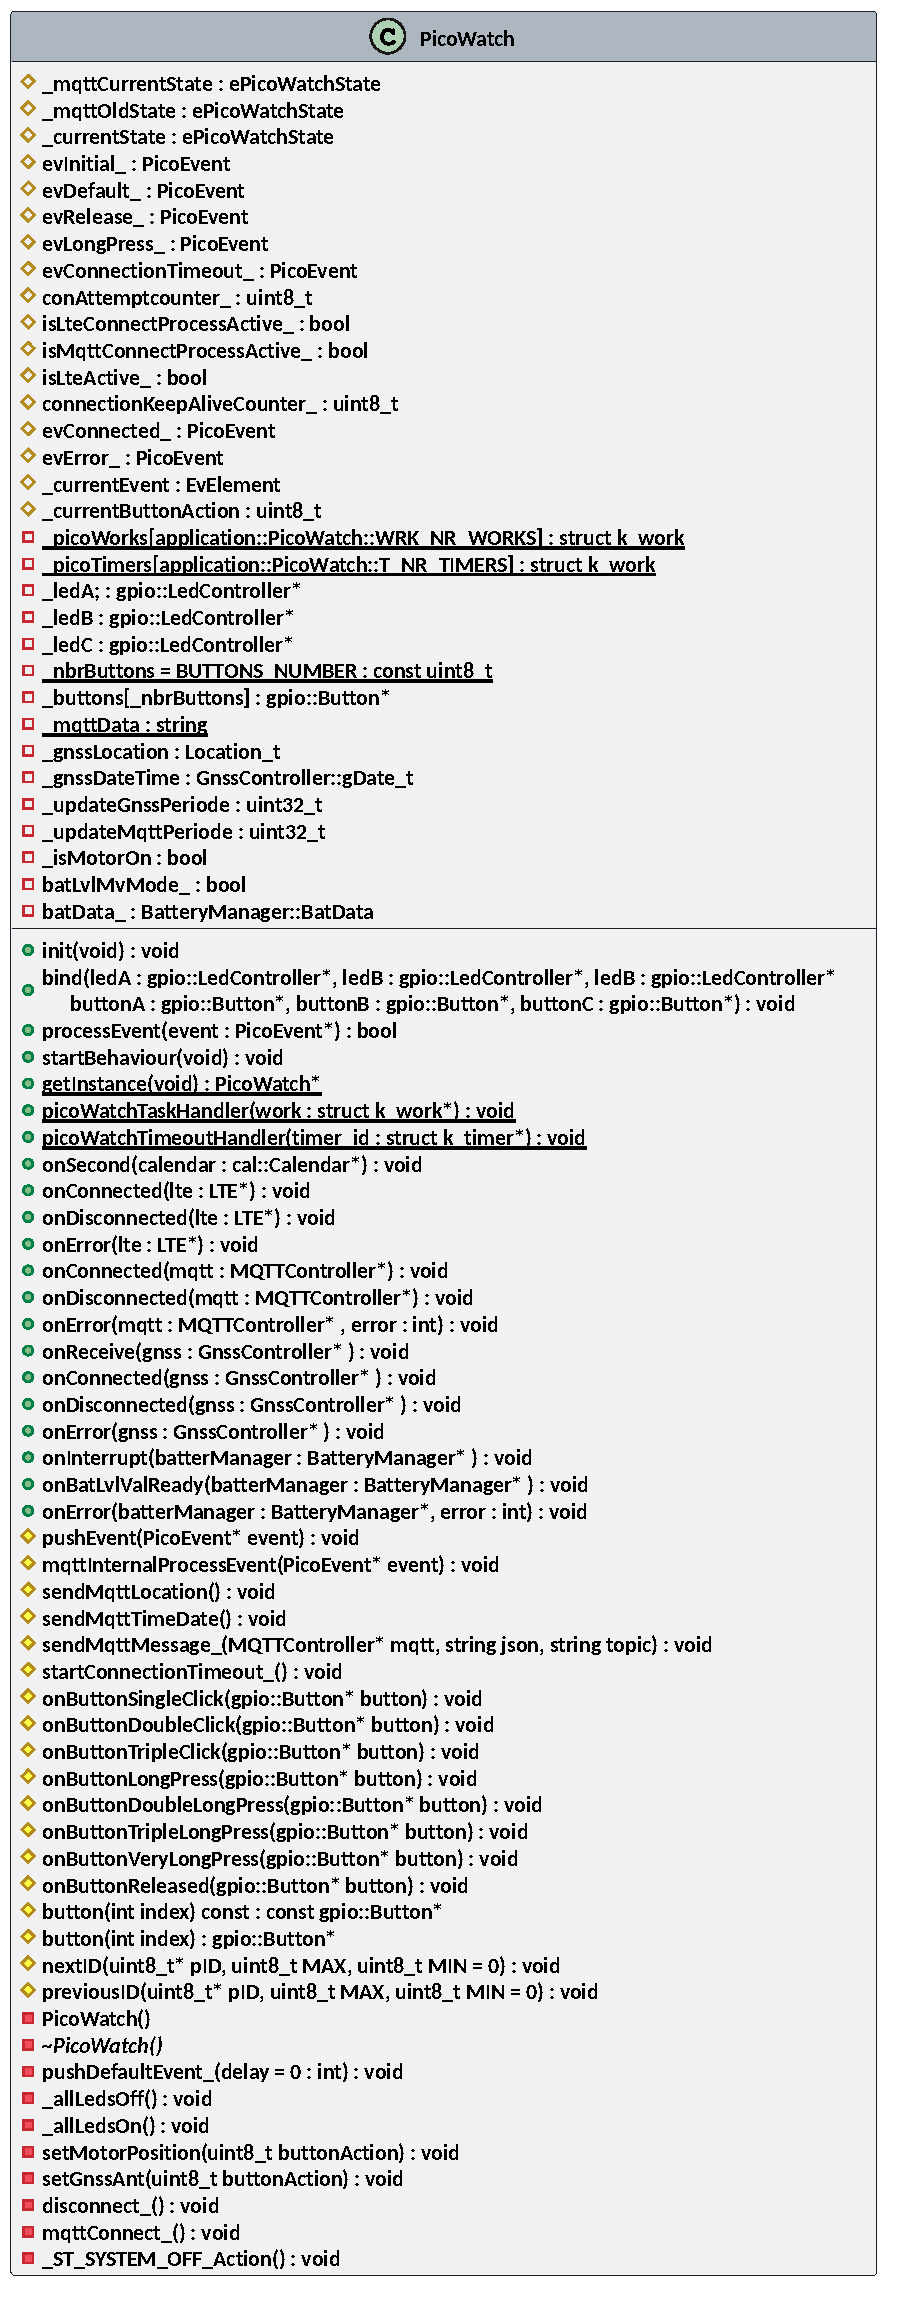
\includegraphics[width=0.6\textwidth]{Include/Figure/software/class/picowatch_small_1.pdf}
	\caption{\textit{PicoWatch} Class Diagram - Part 2}
	\label{fig:picowatch_small_2}
\end{figure}

\subsection{\textit{PicoWatch} State Diagram}

Figure \ref{fig:picoWatch} illustrates the state diagram of \textit{PicoWatch} class: 

\begin{figure}[H]
	\centering
	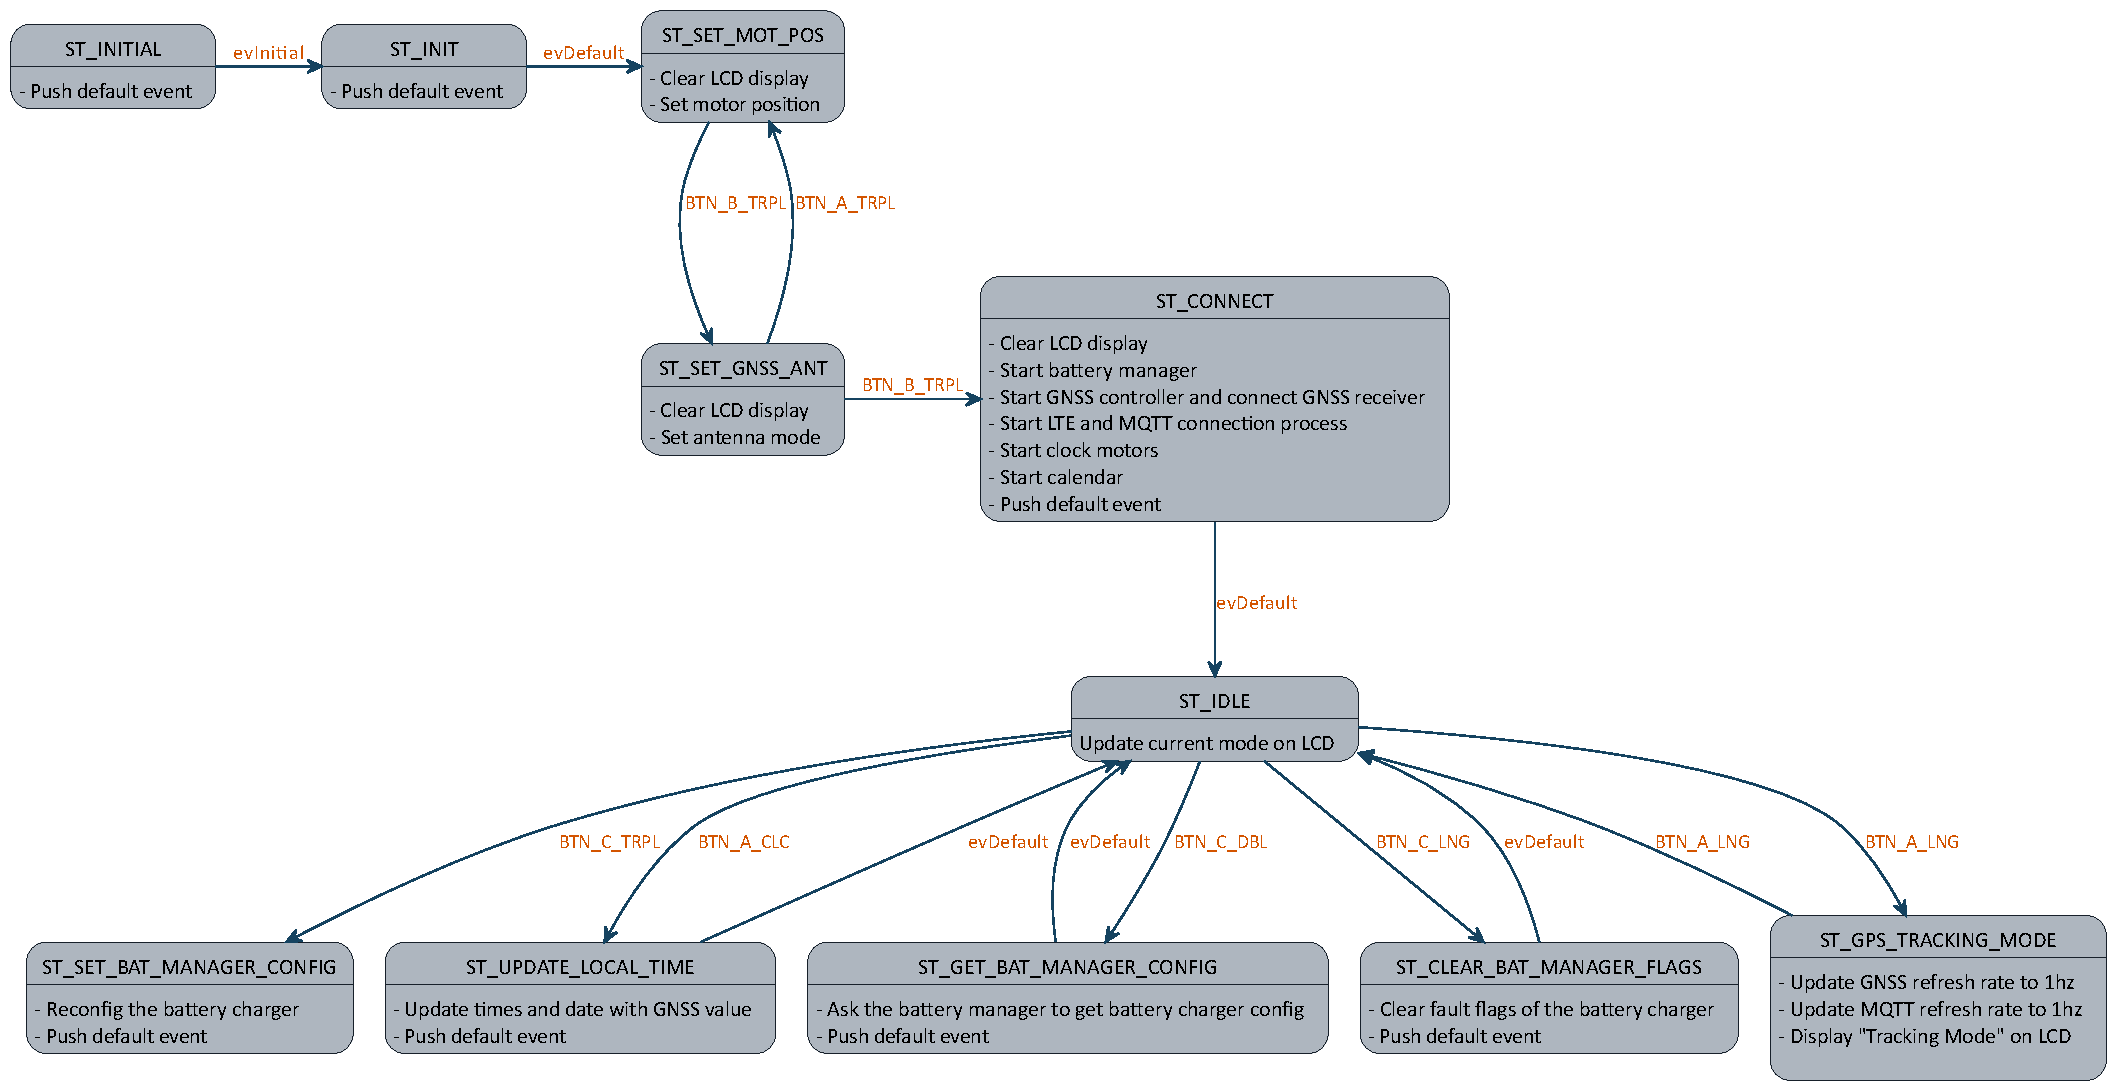
\includegraphics[width=1\textwidth]{Include/Figure/software/state/picoWatch.pdf}
	\caption{\textit{PicoWatch} State Diagram}
	\label{fig:picoWatch}
\end{figure}

\subsection{\textit{PicoWatch - MQTT} Internal State Diagram}

Figure \ref{fig:picoWatchInternal} illustrates \textit{PicoWatch - MQTT} internal state diagram: 

\begin{figure}[H]
	\centering
	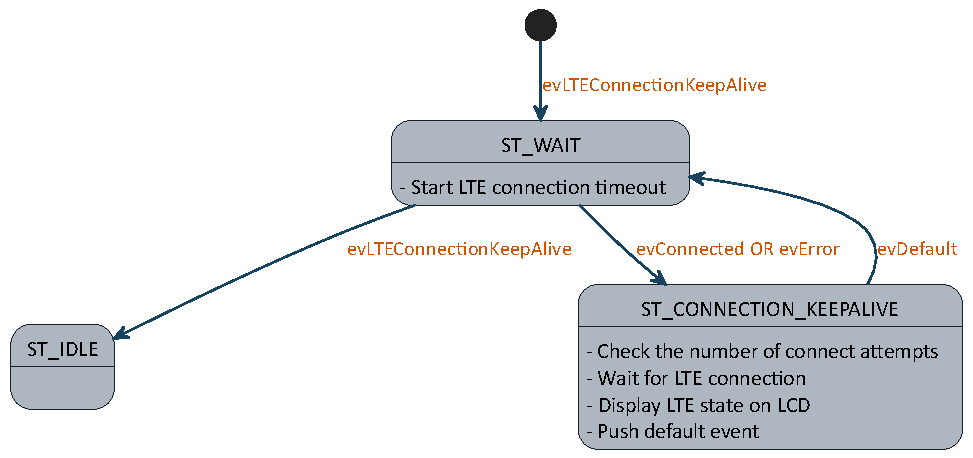
\includegraphics[width=1\textwidth]{Include/Figure/software/state/picoWatchInternal.pdf}
	\caption{\textit{PicoWatch - MQTT} State Diagram}
	\label{fig:picoWatchInternal}
\end{figure}


\begin{landscape}
\subsection{\textit{PicoWatch} - Common Name-space - Class Diagram}

Figure \ref{fig:picoWatchCommon} illustrates the diagram of \textit{PicoWatch} \textit{common} classes from \textit{LTEWatch} application: 

\begin{figure}[H]
	\centering
	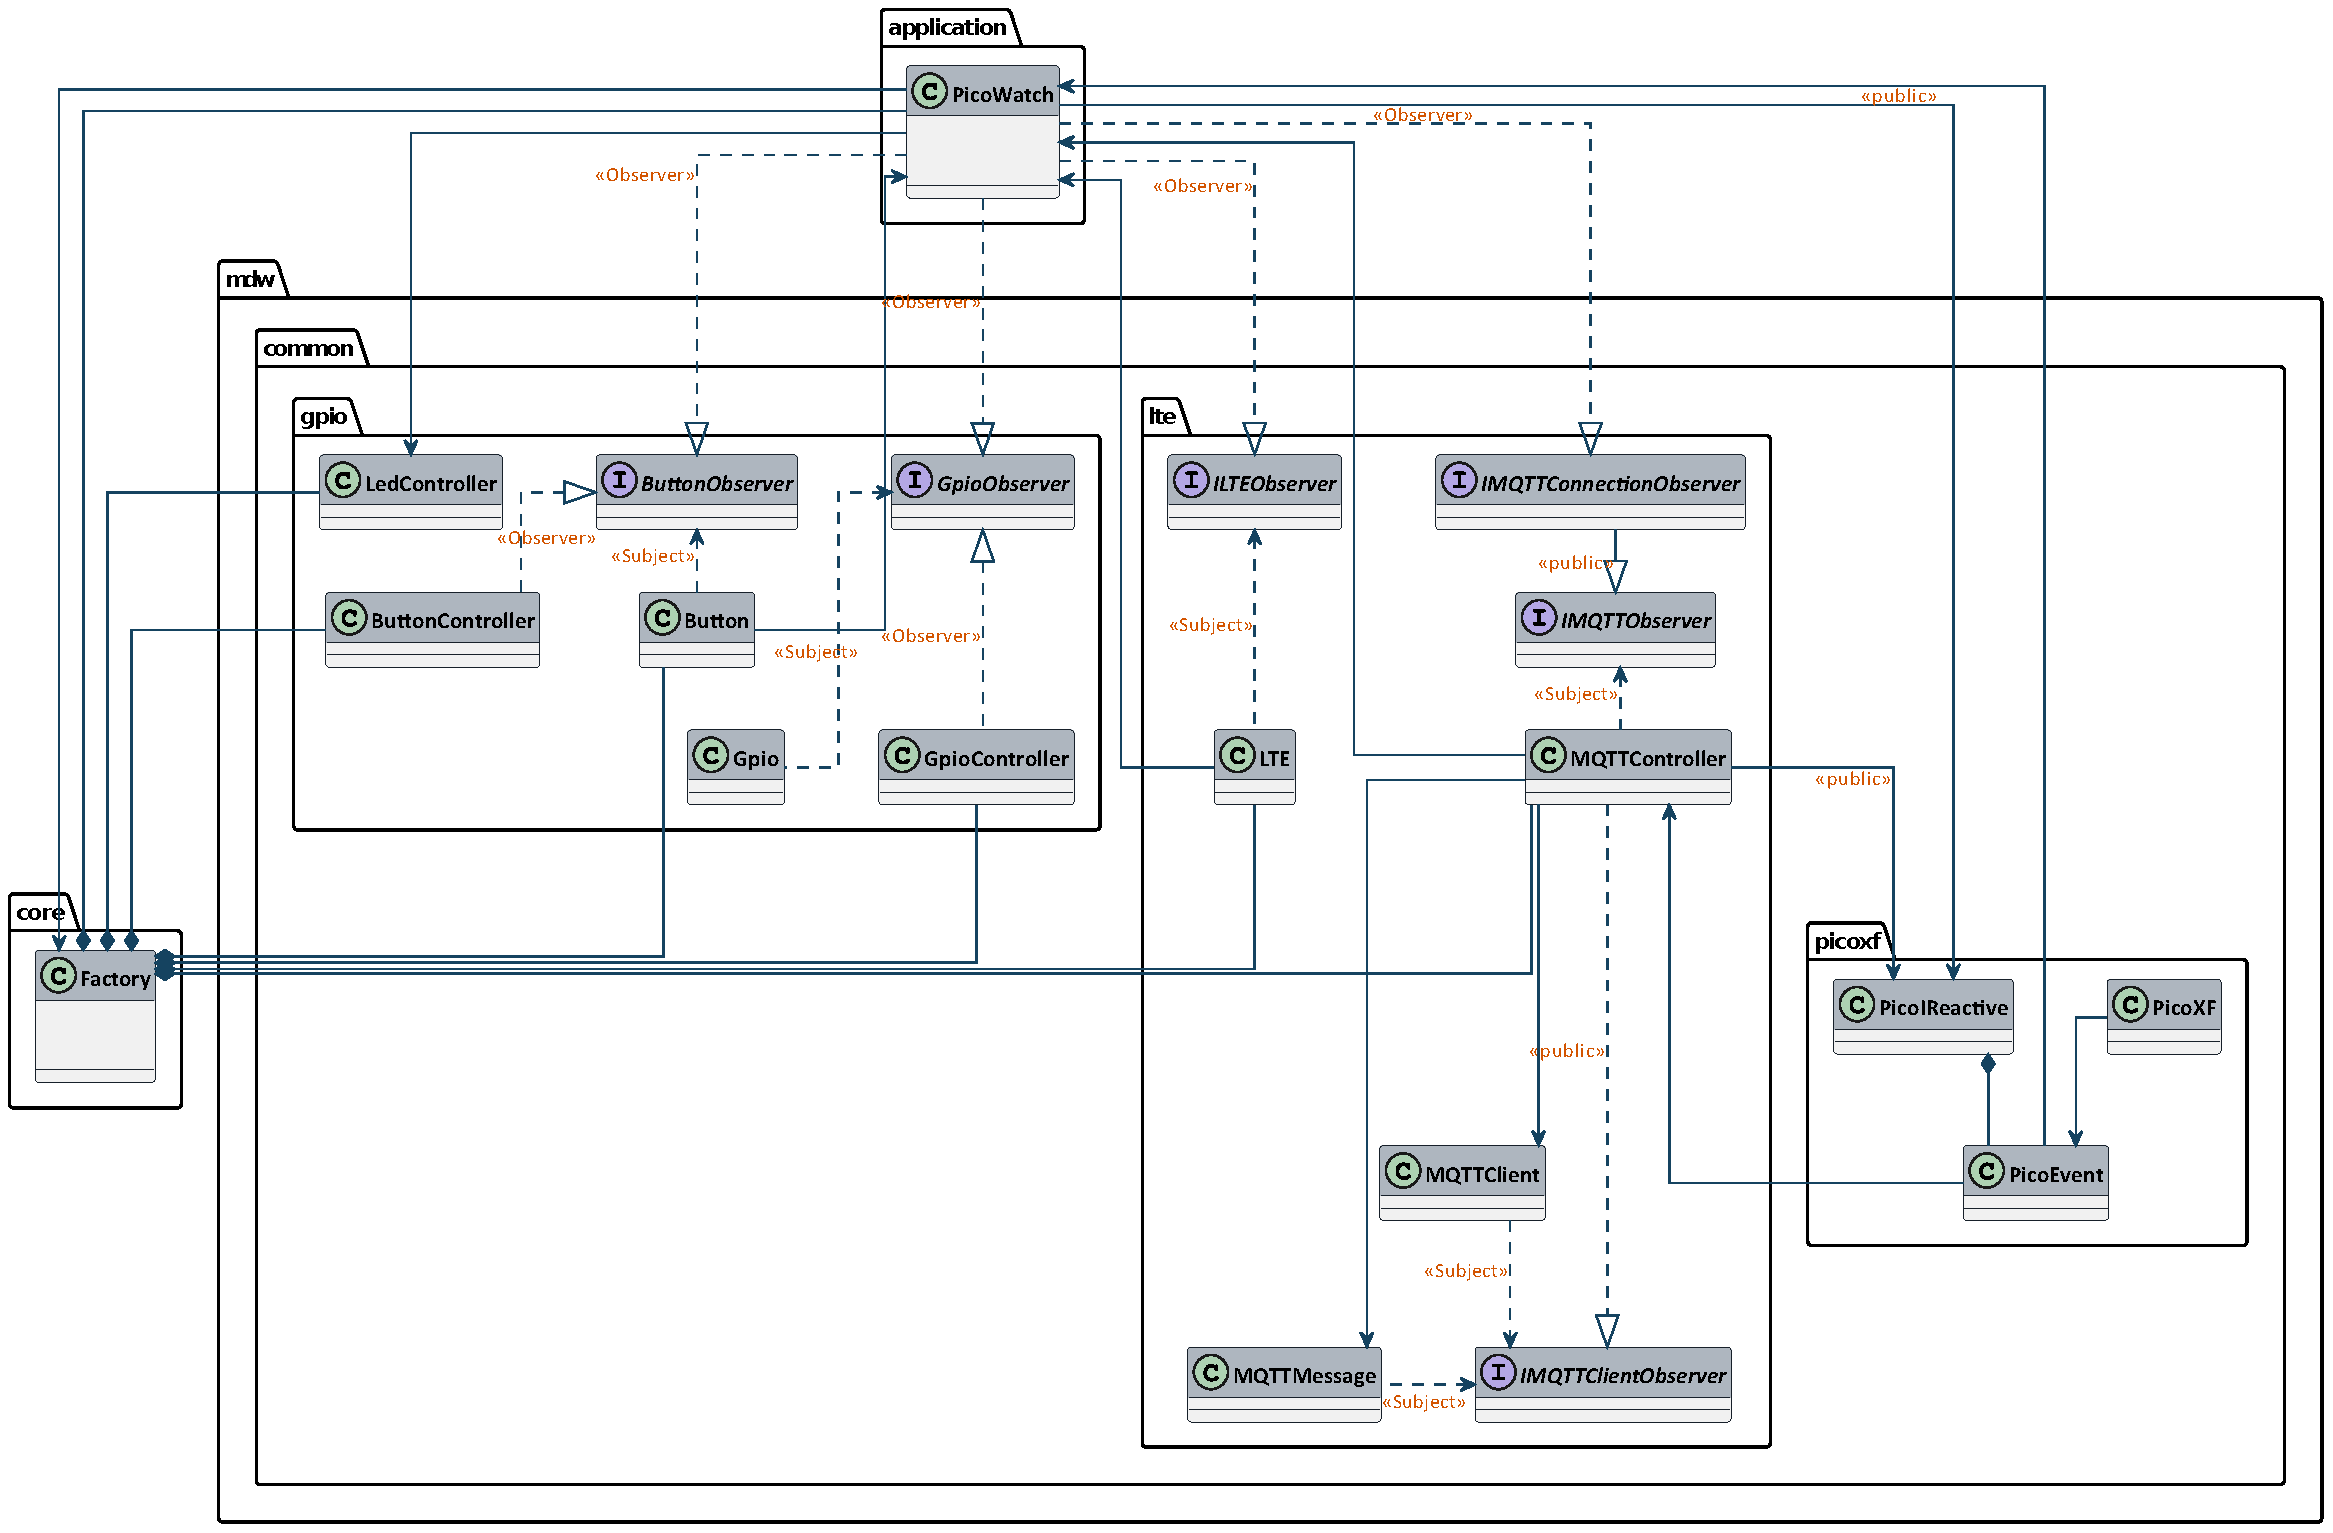
\includegraphics[width=1.2\textwidth]{Include/Figure/software/class/picoWatchCommon.pdf}
	\caption{Name-space : \textit{common} from \textit{PicoWatch} Application}
	\label{fig:picoWatchCommon}
\end{figure}
\end{landscape}

\begin{landscape}

\subsection{\textit{PicoWatch} - Partners Name-space - Class Diagram}

Figure \ref{fig:picoWatchPartner} illustrates the diagram of \textit{PicoWatch} \textit{partners} classes from \textit{LTEWatch} application: 


\begin{figure}[H]
	\centering
	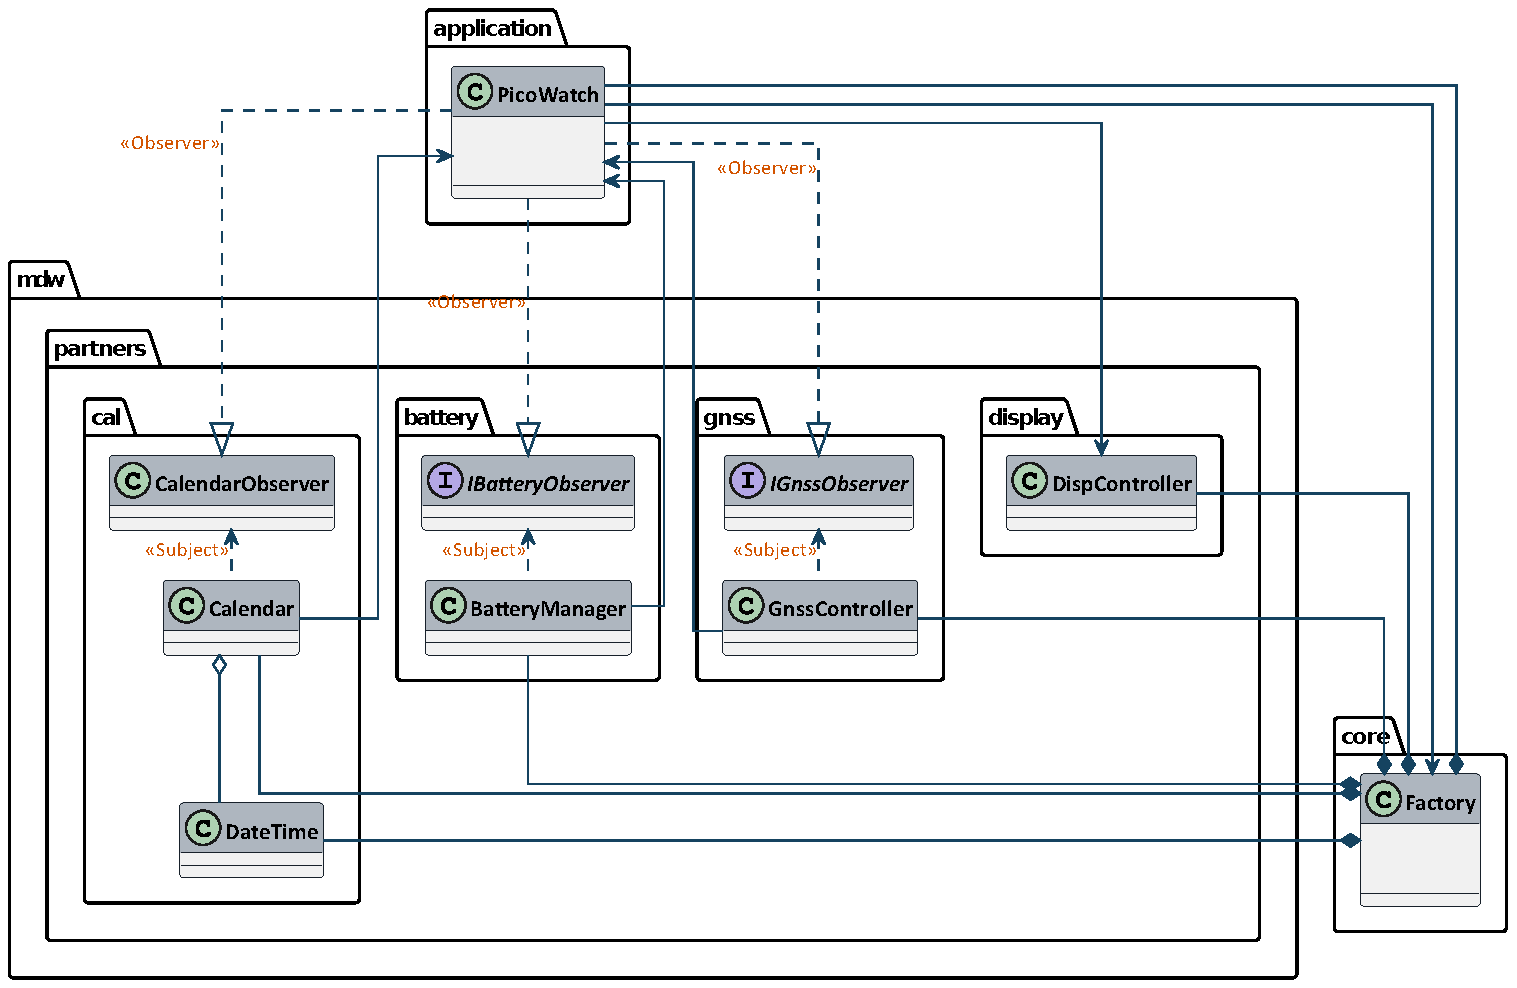
\includegraphics[width=1.25\textwidth]{Include/Figure/software/class/picoWatchPartner.pdf}
	\caption{Name-space : \textit{partners} from \textit{PicoWatch} Application}
	\label{fig:picoWatchPartner}
\end{figure}
\end{landscape}

\begin{landscape}
\section{Motor Driver}
\subsection{Motor driver Classes Diagram}

Figure \ref{fig:motorDriving} illustrates the architecture of classes in relation with motor driver: 

\begin{figure}[H]
	\centering
	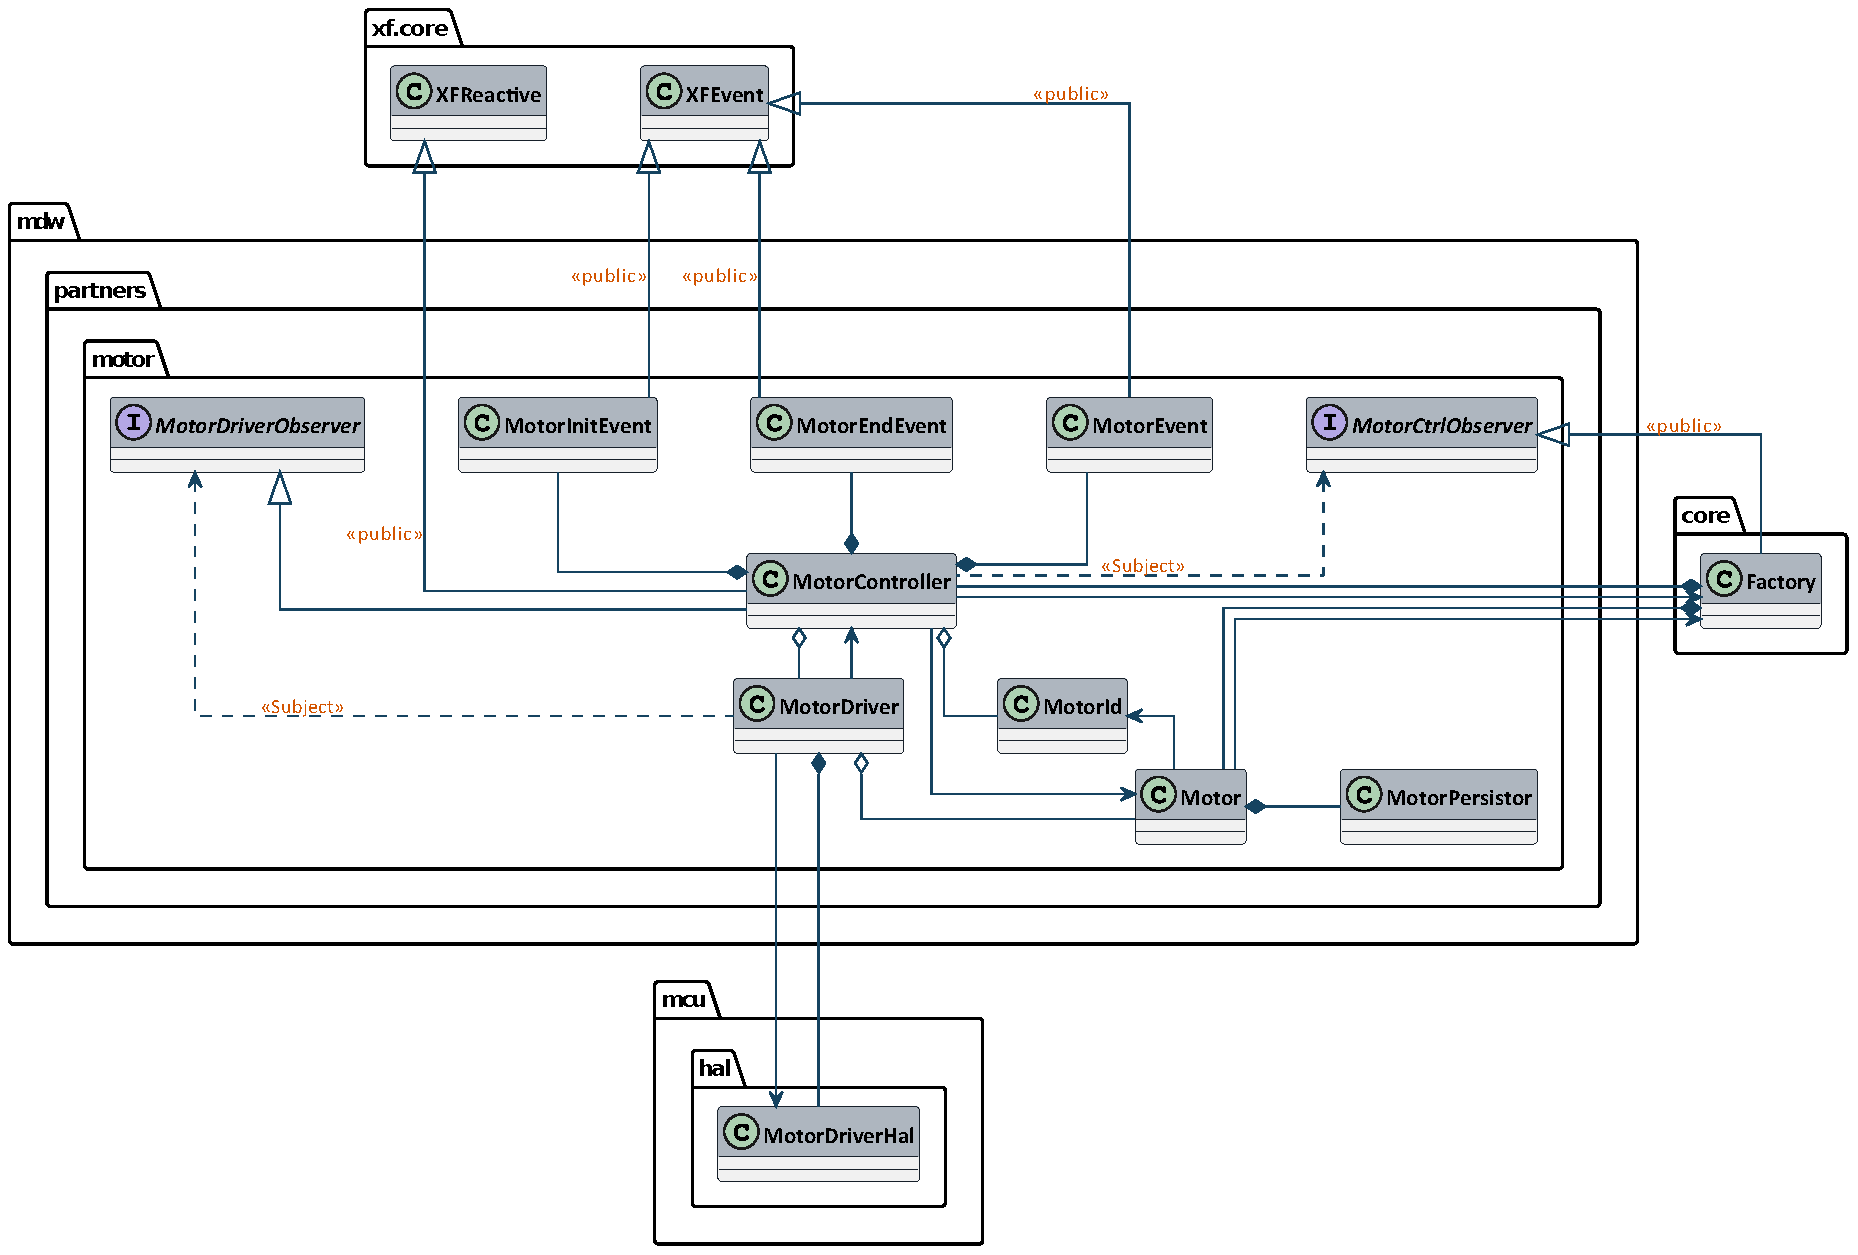
\includegraphics[width=1.1\textwidth]{Include/Figure/software/class/motorDriving.pdf}
	\caption{Motor driver related classes Diagram}
	\label{fig:motorDriving}
\end{figure}
\end{landscape}

\section{Pico XF}
\subsection{\textit{PicoXF} Class Diagram}

Figure \ref{fig:picoxf} illustrates the class diagram of \textit{PicoXF}: 

\begin{figure}[H]
	\centering
	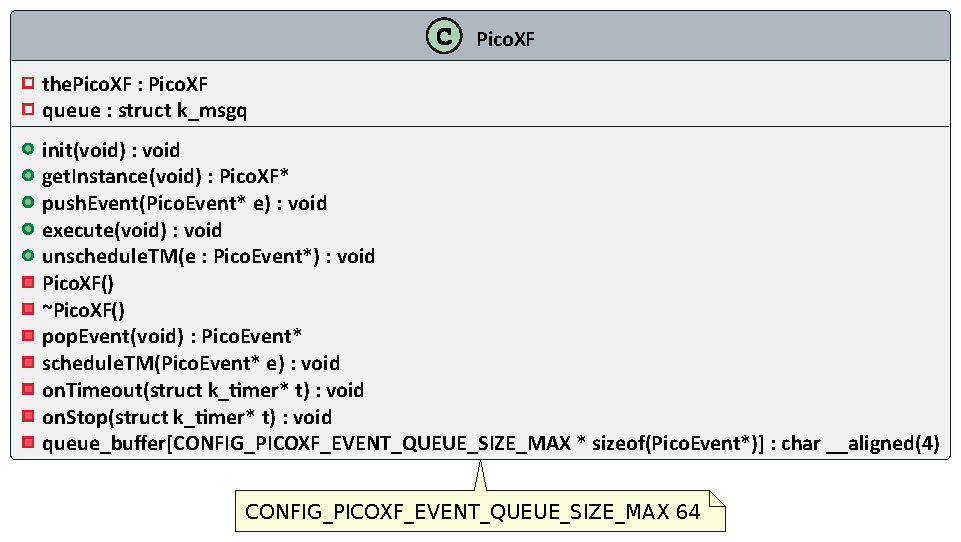
\includegraphics[width=1\textwidth]{Include/Figure/software/class/picoxf.pdf}
	\caption{\textit{PicoXF} Class Diagram}
	\label{fig:picoxf}
\end{figure}

\subsection{\textit{PicoIReactive} Class Diagram}

Figure \ref{fig:PicoIReactive} illustrates the class diagram of \textit{PicoIReactive}: 

\begin{figure}[H]
	\centering
	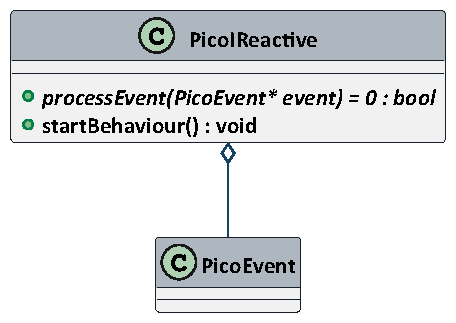
\includegraphics[width=0.4\textwidth]{Include/Figure/software/class/PicoIReactive.pdf}
	\caption{\textit{PicoIReactive} Class Diagram}
	\label{fig:PicoIReactive}
\end{figure}

\pagebreak
\subsection{\textit{PicoEvent} Class Diagram}
Figure \ref{fig:picoevent} illustrates the diagram of \textit{PicoEvent} class from \textit{LTEWatch} application: 

\begin{figure}[H]
	\centering
	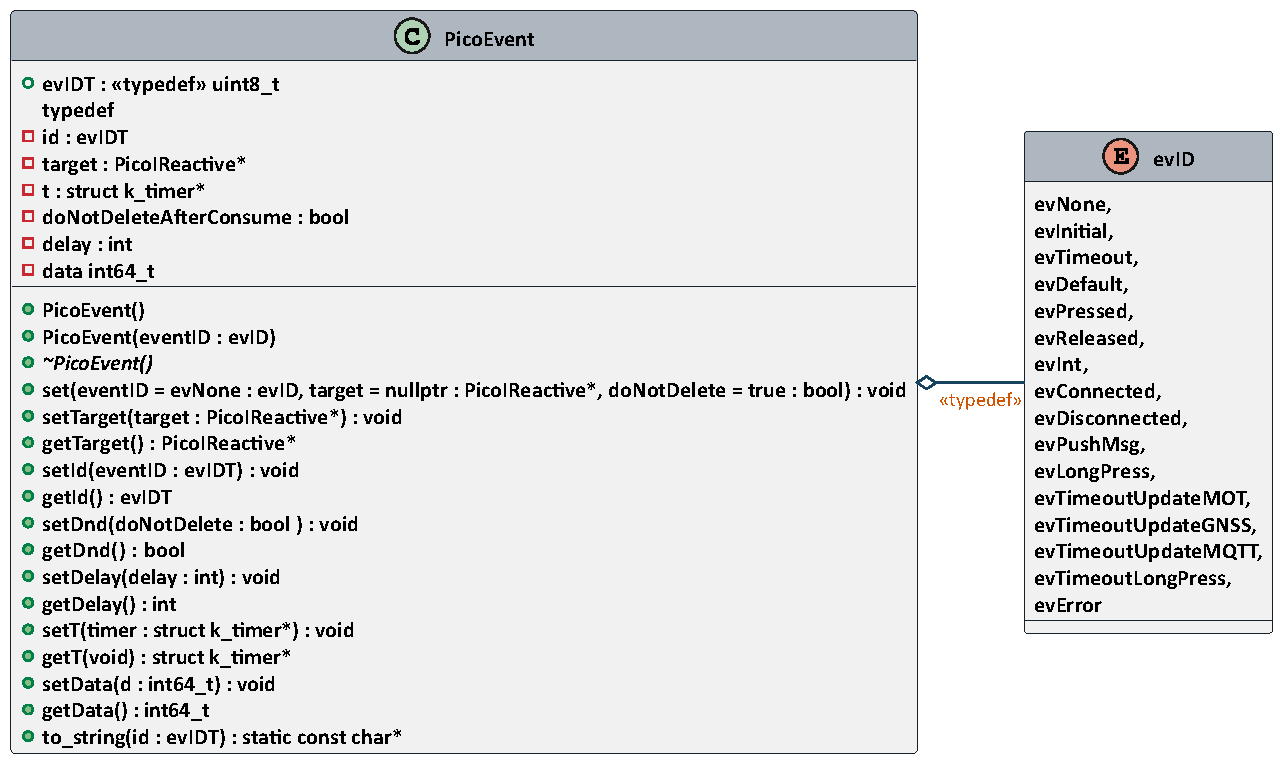
\includegraphics[width=1\textwidth]{Include/Figure/software/class/picoevent.pdf}
	\caption{\textit{PicoEvent} Class Diagram}
	\label{fig:picoevent}
\end{figure}

\end{document}
